\documentclass[11pt,spanish]{article}

% --- Idioma y codificación ---
\usepackage[spanish,es-tabla]{babel}
\usepackage[T1]{fontenc}
\usepackage[utf8]{inputenc}

% --- Matemáticas ---
\usepackage{amsmath}

% --- Tablas, enlaces y elementos visuales ---
\usepackage{array}
\usepackage{tabularx}
\usepackage{booktabs}
\usepackage{longtable}
\usepackage{graphicx}
\usepackage{float}
\usepackage{xcolor}
\usepackage{tikz}
\usetikzlibrary{positioning,shapes.geometric,arrows.meta,calc}
\usepackage{enumitem}
\usepackage{ragged2e}
\usepackage[hidelinks]{hyperref}

\newcolumntype{Y}{>{\RaggedRight\arraybackslash}X}
\renewcommand{\arraystretch}{1.22}
\setlength{\LTpre}{0.5em}
\setlength{\LTpost}{0.5em}
\sloppy
\makeatletter
\newcommand{\SyncPageBuilderDimensions}{%
\global\vsize=\textheight
\global\@colroom=\textheight
\global\@colht=\textheight
}
\makeatother

\newenvironment{widepage}{%
\clearpage
\hypersetup{pageanchor=false}%
\paperwidth=297mm
\paperheight=210mm
\pdfpagewidth=297mm
\pdfpageheight=210mm
\newgeometry{left=2.7cm,right=2.7cm,top=2.7cm,bottom=2.7cm}%
\setlength{\textwidth}{243mm}%
\setlength{\textheight}{156mm}%
\setlength{\linewidth}{\textwidth}%
\setlength{\columnwidth}{\textwidth}%
\hsize=\textwidth
\setlength{\headwidth}{\textwidth}%
\SyncPageBuilderDimensions
\pagestyle{widefancy}%
}{%
\clearpage
\paperwidth=210mm
\paperheight=297mm
\pdfpagewidth=210mm
\pdfpageheight=297mm
\restoregeometry
\setlength{\textwidth}{156mm}%
\setlength{\textheight}{243mm}%
\setlength{\linewidth}{\textwidth}%
\setlength{\columnwidth}{\textwidth}%
\hsize=\textwidth
\setlength{\headwidth}{\textwidth}%
\SyncPageBuilderDimensions
\hypersetup{pageanchor=true}%
\pagestyle{fancy}%
}

% --- Márgenes / papel ---
\usepackage{geometry}
\geometry{a4paper, margin=2.7cm}

% --- Encabezado y pie de página ---
\usepackage[myheadings]{fancyhdr}
\setlength{\headheight}{30pt}
\setlength{\footskip}{30pt}
\usepackage{lastpage}

\pagestyle{fancy}
\fancyhf{} % limpia header/footer

% Header/footer
\newcommand{\DocHeaderLeft}{Proyecto 01}
\newcommand{\DocHeaderRight}{Aseguramiento de la calidad del software}
\newcommand{\DocFooterRight}{Página~\thepage\ de~\pageref{LastPage}}

\fancyhead[L]{\DocHeaderLeft}
\fancyhead[R]{\DocHeaderRight}
\renewcommand{\footrulewidth}{0.4pt}
\fancyfoot[R]{\DocFooterRight}

\fancypagestyle{widefancy}{%
\fancyhf{}%
\fancyhead[L]{\DocHeaderLeft}%
\fancyhead[R]{\DocHeaderRight}%
\renewcommand{\headrulewidth}{0.4pt}%
\renewcommand{\footrulewidth}{0.4pt}%
\fancyfoot[R]{\DocFooterRight}%
}

% --- Interlineado ---
\linespread{1.2}

% --- Metadatos ---
\title{Informe final de aseguramiento de la calidad aplicado a Claustrum}
\author{Mauricio González Prendas, Isaac Jiménez Blanco y Armando Castro Palma}
\date{14 de junio de 2026}

\begin{document}
\hypersetup{pageanchor=false}

% =========================
% Portada
% =========================
\begin{titlepage}
\thispagestyle{empty}
\centering

{\bfseries \huge Instituto Tecnológico de Costa Rica \par}
\vspace{0.25cm}
{\LARGE Campus Tecnológico Central Cartago \par}

\vfill

{\huge Informe final de aseguramiento de la calidad aplicado a Claustrum \par}

\vfill

{\bfseries \LARGE Profesora: \par}
{\Large Alicia Marcela Salazar Hernandez \par}

\vfill

{\bfseries \LARGE Estudiantes: \par}
{\Large Mauricio González Prendas: 2024143009 \par}
{\Large Isaac Jiménez Blanco: 2024202804 \par}
{\Large Armando Castro Palma: 2023219038 \par}

\vfill

{\bfseries\LARGE Fecha: \par}
{\Large 14 de junio de 2026 \par}

\vfill

{\LARGE I Semestre \par}
{\LARGE 2026 \par}

\end{titlepage}

% =========================
% Índice
% =========================
\pagenumbering{roman}
\pagestyle{empty}
\tableofcontents
\clearpage
\pagenumbering{arabic}
\hypersetup{pageanchor=true}
\pagestyle{fancy}

% =========================
% Contenido
% =========================
\section{Introducción}

El presente informe documenta el proceso de aseguramiento de la calidad aplicado a Claustrum, una aplicación web orientada a estudiantes del Instituto Tecnológico de Costa Rica. El trabajo se concentró en rutas funcionales representativas del uso académico cotidiano, específicamente el creador de horarios, el panel de resumen, el módulo de profesores y reseñas, la autenticación, el onboarding académico y la malla curricular. A partir de este alcance se diseñaron requisitos, criterios de aceptación, casos de prueba, evidencias, métricas y un registro formal de defectos.

La finalidad del documento no se limita a enumerar pruebas ejecutadas, sino que integra el plan de calidad, la matriz de trazabilidad, los casos de prueba, los defectos encontrados y la evaluación final en una visión unificada del estado del sistema evaluado. Por esa razón, los resultados se interpretan en función del impacto sobre los requisitos seleccionados, la experiencia del usuario, la seguridad observable, el rendimiento y la mantenibilidad de los flujos analizados.

El proceso combinó pruebas manuales y automatizadas mediante Playwright para flujos de extremo a extremo, Vitest para lógica unitaria de calendario, Postman y Newman para validación de API, Lighthouse para rendimiento y accesibilidad, ApacheBench para carga ligera y revisión manual para criterios de usabilidad, funcionalidad y seguridad. Esta combinación permitió obtener evidencia suficiente para sustentar conclusiones sobre cada módulo dentro del alcance definido.

\section{Contexto del proyecto}

Claustrum es una aplicación web de apoyo académico que permite a estudiantes gestionar horarios, consultar información curricular, revisar datos de cursos y profesores, y utilizar funciones de seguimiento académico. En el contexto de este proyecto, el sistema fue tratado como una aplicación real en evolución, por lo que las pruebas se orientaron a validar flujos de usuario observables y atributos de calidad relevantes para una entrega académica formal.

El alcance incluyó las rutas \texttt{schedule}, \texttt{overview}, \texttt{professors}, \texttt{auth}, \texttt{onboarding} y \texttt{curriculum}, considerando que \texttt{schedule} es importante para la creación y persistencia de horarios académicos, \texttt{overview} incide en la primera percepción de rendimiento y \texttt{professors} integra consulta de información, reseñas, validación de formularios y consumo de API. Además, las rutas \texttt{auth} y \texttt{onboarding} fueron incluidas porque condicionan el acceso al sistema, mientras que \texttt{curriculum} se evaluó por su valor informativo y por requerir navegación clara.

Quedaron fuera del alcance la ruta de evaluaciones en PDF, la moderación, la documentación interna, las políticas, la infraestructura de integración y despliegue continuo, y el pipeline de datos en Python. Estas exclusiones respondieron a la necesidad de concentrar los recursos del equipo en flujos directamente relacionados con la experiencia del estudiante y con evidencia ejecutable dentro del tiempo disponible.

\section{Objetivos}

\subsection{Objetivo general}

Ejecutar un proceso completo de aseguramiento de la calidad sobre módulos seleccionados de Claustrum, mediante pruebas funcionales, no funcionales, automatizadas y manuales que permitan evaluar el cumplimiento de requisitos y documentar defectos con evidencia verificable.

\subsection{Objetivos específicos}

\begin{enumerate}[label=\arabic*.]
    \item Analizar requisitos funcionales y no funcionales asociados a los módulos seleccionados.
    \item Diseñar casos de prueba con trazabilidad hacia los requisitos definidos.
    \item Ejecutar pruebas estáticas, dinámicas, funcionales, de integración, sistema, aceptación, seguridad, rendimiento y usabilidad según el módulo correspondiente.
    \item Registrar defectos con severidad, prioridad, pasos de reproducción, resultado esperado, resultado actual y evidencia.
    \item Interpretar los resultados obtenidos para formular conclusiones y recomendaciones sustentadas.
\end{enumerate}

\section{Plan de calidad del proyecto}

El plan de calidad definió el alcance operativo, los responsables, los requisitos seleccionados, la estrategia de pruebas, las herramientas, los recursos y los criterios de aceptación, con el propósito de establecer una base común para que las pruebas no dependieran únicamente de exploración informal, sino de una estructura controlada y trazable.

\subsection{Alcance y responsabilidades}

\begin{table}[H]
\centering
\caption{Módulos incluidos en el alcance de calidad}
\label{tab:alcance-incluido}
\begin{tabularx}{\textwidth}{p{4.2cm} p{2.8cm} Y}
\toprule
\textbf{Módulo} & \textbf{Responsable} & \textbf{Pruebas principales} \\
\midrule
Ruta \texttt{schedule}, creador de horarios & Mauricio & Pruebas funcionales, integración, extremo a extremo y validación de comportamiento ante conflictos. \\
Ruta \texttt{overview}, panel de resumen & Mauricio & Pruebas de rendimiento, carga ligera, usabilidad y validación visual. \\
Ruta \texttt{professors}, reseñas de profesores & Isaac & Pruebas funcionales, API, seguridad, validaciones negativas y aceptación de usuario. \\
Ruta \texttt{auth}, autenticación & Armando & Pruebas funcionales, negativas, seguridad y control de acceso. \\
Ruta \texttt{onboarding}, configuración inicial & Armando & Pruebas funcionales y de integración sobre el estado académico inicial. \\
Ruta \texttt{curriculum}, malla curricular & Armando & Pruebas funcionales, usabilidad, accesibilidad y navegación autenticada. \\
\bottomrule
\end{tabularx}
\end{table}

La distribución de responsabilidades permitió cubrir módulos con naturaleza distinta, ya que el bloque de horarios y rendimiento del panel de resumen, el módulo de reseñas y seguridad de entradas, y las rutas de autenticación, onboarding, navegación y malla curricular requerían estrategias de prueba diferentes. Esta separación ayudó a mantener evidencia organizada y a asociar cada requisito con un responsable claro.

\begin{table}[H]
\centering
\caption{Elementos excluidos del alcance}
\label{tab:alcance-excluido}
\begin{tabularx}{\textwidth}{p{4.5cm} Y}
\toprule
\textbf{Elemento excluido} & \textbf{Justificación} \\
\midrule
Ruta \texttt{evaluations} & Se excluyó por el manejo de archivos PDF y por requerir validaciones adicionales fuera del flujo principal evaluado. \\
Ruta \texttt{moderation} & Corresponde a un flujo administrativo que no era esencial para la perspectiva del usuario estudiante. \\
Documentación interna y políticas & Son contenidos informativos sin interacción crítica dentro del alcance definido. \\
CI/CD & Pertenece a infraestructura de desarrollo y despliegue, no a funcionalidad directa del usuario final. \\
Pipeline de datos Python & Es una herramienta interna que no se utiliza directamente en los flujos de estudiante evaluados. \\
\bottomrule
\end{tabularx}
\end{table}

\subsection{Requisitos seleccionados}

\begin{table}[H]
\centering
\caption{Requisitos funcionales y no funcionales evaluados}
\label{tab:requisitos}
\begin{tabularx}{\textwidth}{p{1.8cm} p{2.4cm} Y p{2.5cm}}
\toprule
\textbf{ID} & \textbf{Tipo} & \textbf{Descripción} & \textbf{Responsable} \\
\midrule
RF-M1 & Funcional & El usuario autenticado puede crear, guardar y cargar un horario académico. & Mauricio \\
RNF-M1 & No funcional & El panel de resumen debe cargar en menos de 2 segundos en una conexión normal. & Mauricio \\
RF-I1 & Funcional & El usuario puede consultar y enviar una reseña de profesor con los campos obligatorios. & Isaac \\
RNF-I1 & No funcional & El módulo de reseñas debe rechazar entradas maliciosas o inválidas. & Isaac \\
RF-A1 & Funcional & El usuario puede iniciar sesión y completar el onboarding académico. & Armando \\
RNF-A1 & No funcional & El usuario puede llegar a las rutas \texttt{overview}, \texttt{schedule}, \texttt{curriculum} y \texttt{professors} en máximo 3 clics desde la aplicación autenticada. & Armando \\
\bottomrule
\end{tabularx}
\end{table}

\subsection{Estrategia de pruebas y herramientas}

La estrategia combinó técnicas complementarias, de modo que las pruebas funcionales y de integración se usaron para verificar que los flujos principales produjeran el resultado esperado, mientras que las pruebas negativas se aplicaron a credenciales inválidas, campos obligatorios vacíos, conflictos de horario y entradas maliciosas. A su vez, las pruebas de rendimiento y carga se enfocaron en el panel de resumen, y las pruebas de accesibilidad y usabilidad revisaron la navegación autenticada y la malla curricular.

\begin{table}[H]
\centering
\caption{Herramientas utilizadas durante la evaluación}
\label{tab:herramientas}
\begin{tabularx}{\textwidth}{p{3.5cm} Y}
\toprule
\textbf{Herramienta} & \textbf{Uso dentro del proyecto} \\
\midrule
oxlint & Revisión estática de código en archivos seleccionados, principalmente en componentes relacionados con horarios y calendario. \\
Vitest & Pruebas unitarias sobre utilidades de calendario y lógica relacionada con horarios. \\
Playwright & Automatización de flujos autenticados y validación de comportamiento de extremo a extremo. \\
Postman y Newman & Ejecución automatizada de pruebas de API para endpoints reales de Supabase RPC asociados al módulo de reseñas. \\
Lighthouse & Medición de rendimiento, accesibilidad, buenas prácticas y SEO en rutas seleccionadas. \\
ApacheBench & Ejecución de carga ligera sobre una ruta principal para observar respuesta básica bajo concurrencia moderada. \\
\bottomrule
\end{tabularx}
\end{table}

\subsection{Métricas y criterios de aceptación}

Las métricas fueron definidas antes de interpretar los resultados, de modo que la evaluación mantuviera criterios explícitos. En la tabla \ref{tab:metricas-aceptacion} se presentan los umbrales utilizados para distinguir aceptación total, aceptación parcial y rechazo.

\begin{table}[H]
\centering
\caption{Métricas y criterios de aceptación}
\label{tab:metricas-aceptacion}
\begin{tabularx}{\textwidth}{p{4.1cm} p{3.2cm} p{3.2cm} Y}
\toprule
\textbf{Métrica} & \textbf{Aceptación total} & \textbf{Aceptación parcial} & \textbf{Rechazo} \\
\midrule
Complejidad ciclomática & Menor o igual a 10 & Entre 11 y 15 & Mayor que 15 \\
Duplicación observable & Menor que 3 \% & Entre 3 \% y 8 \% & Mayor que 8 \% \\
Cobertura en archivos probados & Mayor o igual que 70 \% & Entre 50 \% y 69 \% & Menor que 50 \% \\
Tiempo de carga del panel de resumen & Menor que 2 s & Entre 2 s y 4 s & Mayor que 4 s \\
Accesibilidad Lighthouse & Mayor o igual que 90 & Entre 70 y 89 & Menor que 70 \\
Flujos E2E críticos & Todos pasan & Falla menor documentada & Falla bloqueante \\
Seguridad de entradas & Bloquea o sanitiza & Acepta sin ejecutar el payload & Ejecuta el payload \\
\bottomrule
\end{tabularx}
\end{table}

\section{Matriz de trazabilidad}

La matriz de trazabilidad permitió comprobar que cada requisito tuviera cobertura explícita mediante casos de prueba y, al mismo tiempo, facilitó relacionar los resultados fallidos con defectos concretos, evitando conclusiones generales sin respaldo. La tabla \ref{tab:trazabilidad} muestra la relación entre requisitos, pruebas, resultados y responsables.

\begin{widepage}
{\small
\setlength{\tabcolsep}{3pt}
\begin{longtable}{p{1.5cm} p{5.3cm} p{4.4cm} p{3.4cm} p{1.9cm} p{2.2cm} p{2.1cm}}
\caption{Matriz de trazabilidad de requisitos y pruebas}\label{tab:trazabilidad}\\
\toprule
\textbf{Req.} & \textbf{Descripción} & \textbf{Casos de prueba} & \textbf{Tipo de prueba} & \textbf{Resultado} & \textbf{Defecto} & \textbf{Resp.} \\
\midrule
\endfirsthead
\toprule
\textbf{Req.} & \textbf{Descripción} & \textbf{Casos de prueba} & \textbf{Tipo de prueba} & \textbf{Resultado} & \textbf{Defecto} & \textbf{Resp.} \\
\midrule
\endhead
RF-M1 & El usuario autenticado puede crear, guardar y cargar un horario académico. & CP-M-001, CP-M-002, CP-M-003, CP-M-004, CP-M-006, CP-M-008, CP-M-009 & Funcional, integración, sistema, negativo, unitario y aceptación de usuario & Aprobado & No aplica & Mauricio \\
RNF-M1 & El panel de resumen debe cargar en menos de 2 segundos en una conexión normal. & CP-M-005, CP-M-007 & Rendimiento y carga & Aprobado & No aplica & Mauricio \\
RF-I1 & El usuario puede consultar y enviar una reseña de profesor con los campos obligatorios. & CP-I-001, CP-I-002, CP-I-003, CP-I-004, CP-I-006, CP-I-007 & Funcional, negativo, API y aceptación de usuario & Fallido & DEF-I-001 & Isaac \\
RNF-I1 & El módulo de reseñas debe rechazar entradas maliciosas o inválidas. & CP-I-005, CP-I-006, CP-I-008 & Seguridad y API & Aprobado & No aplica & Isaac \\
RF-A1 & El usuario puede iniciar sesión y completar el onboarding académico. & CP-A-001, CP-A-002, CP-A-003, CP-A-008 & Funcional, negativo, integración y seguridad & Aprobado & DEF-A-001 & Armando \\
RNF-A1 & El usuario puede llegar a las rutas \texttt{overview}, \texttt{schedule}, \texttt{curriculum} y \texttt{professors} en máximo 3 clics desde la aplicación autenticada. & CP-A-004, CP-A-005, CP-A-006, CP-A-007 & Funcional, usabilidad, accesibilidad y aceptación de usuario & Aprobado & No aplica & Armando \\
\bottomrule
\end{longtable}
}
\end{widepage}

Los requisitos RF-M1 y RNF-M1 quedaron cubiertos sin defectos asociados, mientras que RF-I1 y RNF-I1 muestran una diferencia importante entre el comportamiento de consulta y seguridad, que fue aprobado, y el flujo funcional de envío de reseñas, que falló por el defecto DEF-I-001. Por su parte, RF-A1 y RNF-A1 fueron aprobados en los flujos principales de autenticación, onboarding y navegación, aunque RF-A1 mantiene asociado el defecto menor DEF-A-001 por el mensaje mostrado ante credenciales inválidas.

\section{Casos de prueba ejecutados}

Los casos de prueba fueron diseñados con campos uniformes, incluyendo identificador, nombre, objetivo, requisito asociado, tipo, prioridad, precondiciones, datos de prueba, pasos, resultado esperado, resultado obtenido, estado, resultado final y evidencia. Para mantener legibilidad en el informe principal, esta sección presenta una síntesis analítica por módulo y un resumen tabular de resultados, mientras que las evidencias visuales se ubican junto a los flujos correspondientes.

\subsection{Ruta schedule y ruta overview}

La ruta \texttt{schedule} fue evaluada desde el acceso inicial hasta la creación, guardado, carga y validación de conflictos de horario, por lo que las evidencias se presentan en el mismo orden de ejecución para conservar la relación entre el caso, el resultado y la captura correspondiente.

\subsubsection{CP-M-001: acceso al creador de horarios}

El caso CP-M-001 confirmó que un usuario demo autenticado puede acceder al creador de horarios y visualizar el calendario junto con los controles disponibles, lo que respalda el inicio del flujo de creación de horarios porque el usuario llega a la ruta funcional sin errores bloqueantes.

\begin{figure}[H]
\centering
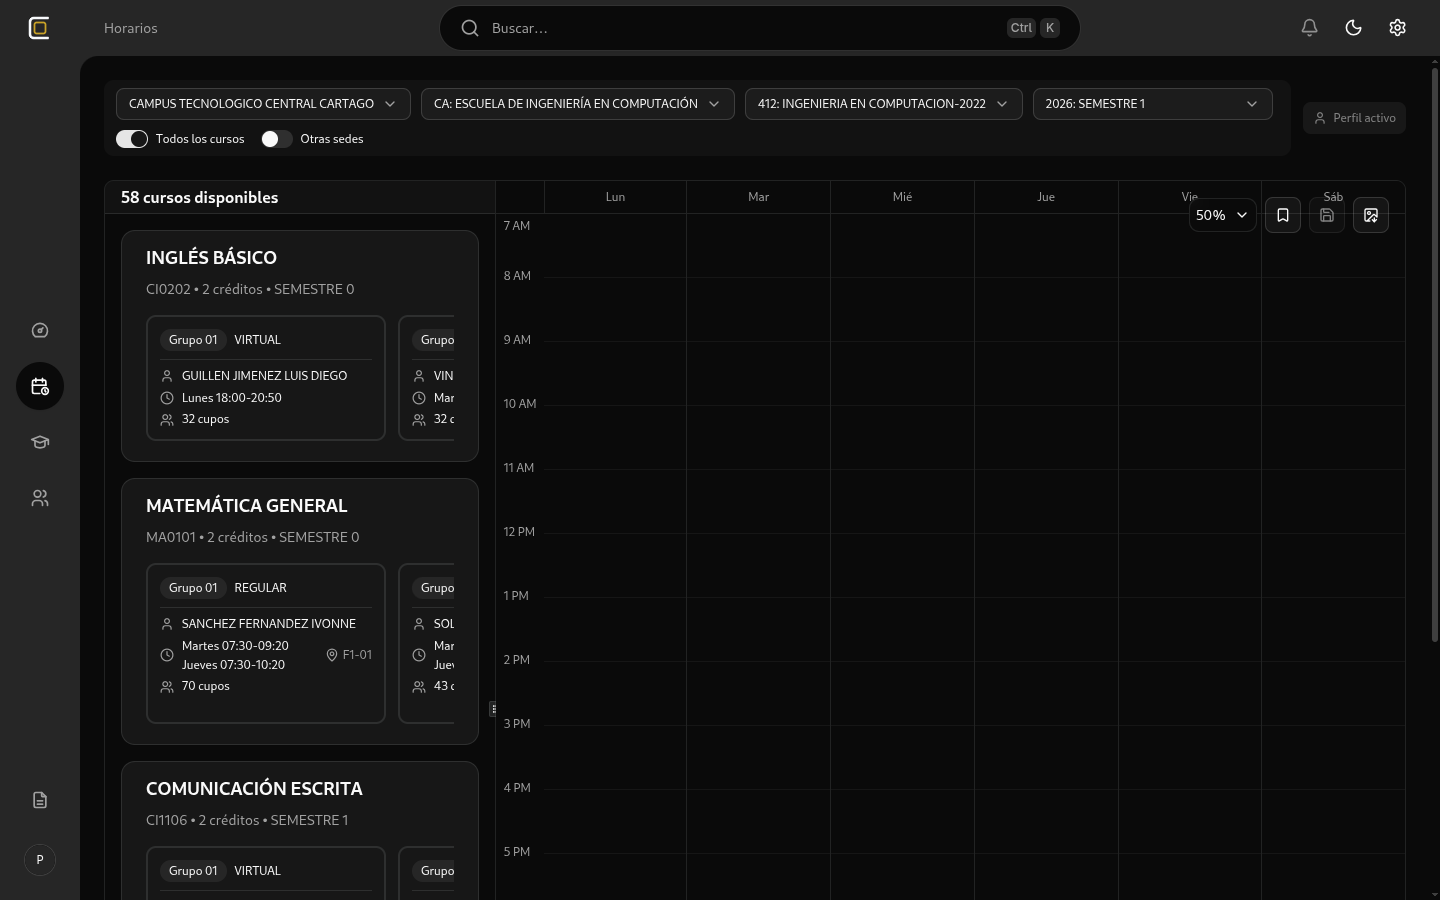
\includegraphics[width=0.92\textwidth]{images/caso-prueba-schedule-acceso-creador.png}
\caption{Acceso autenticado al creador de horarios en la ruta \texttt{schedule}}
\label{fig:schedule-acceso}
\end{figure}

\subsubsection{CP-M-002: agregar grupo al horario}

El caso CP-M-002 validó que el grupo \texttt{MA0101-01} de Matemática General pudiera agregarse al calendario semanal, y la evidencia muestra que la selección se refleja en la vista de horario, lo cual permite verificar que la interacción del usuario modifica correctamente el estado visual del calendario.

\begin{figure}[H]
\centering
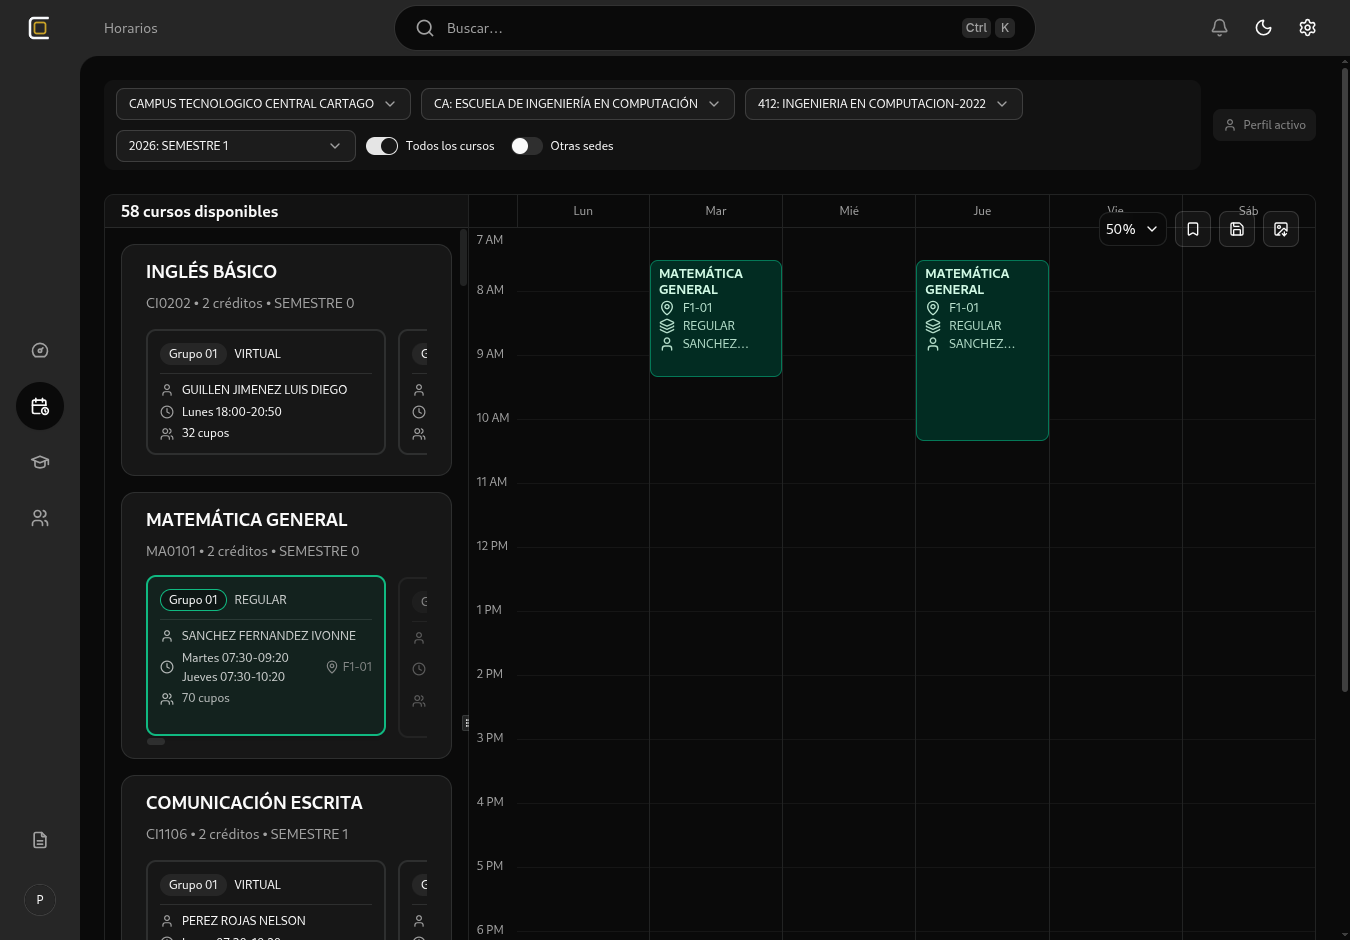
\includegraphics[width=0.92\textwidth]{images/caso-prueba-schedule-agregar-grupo.png}
\caption{Selección de grupo académico y visualización en el calendario semanal}
\label{fig:schedule-agregar}
\end{figure}

\subsubsection{CP-M-003: guardar horario}

El caso CP-M-003 verificó el guardado del horario con el nombre \texttt{Horario QA Mauricio Diurno 2026-06-06}, una prueba relevante porque confirma la transición desde una selección temporal de grupos hacia un registro persistente que el usuario puede reutilizar.

\begin{figure}[H]
\centering
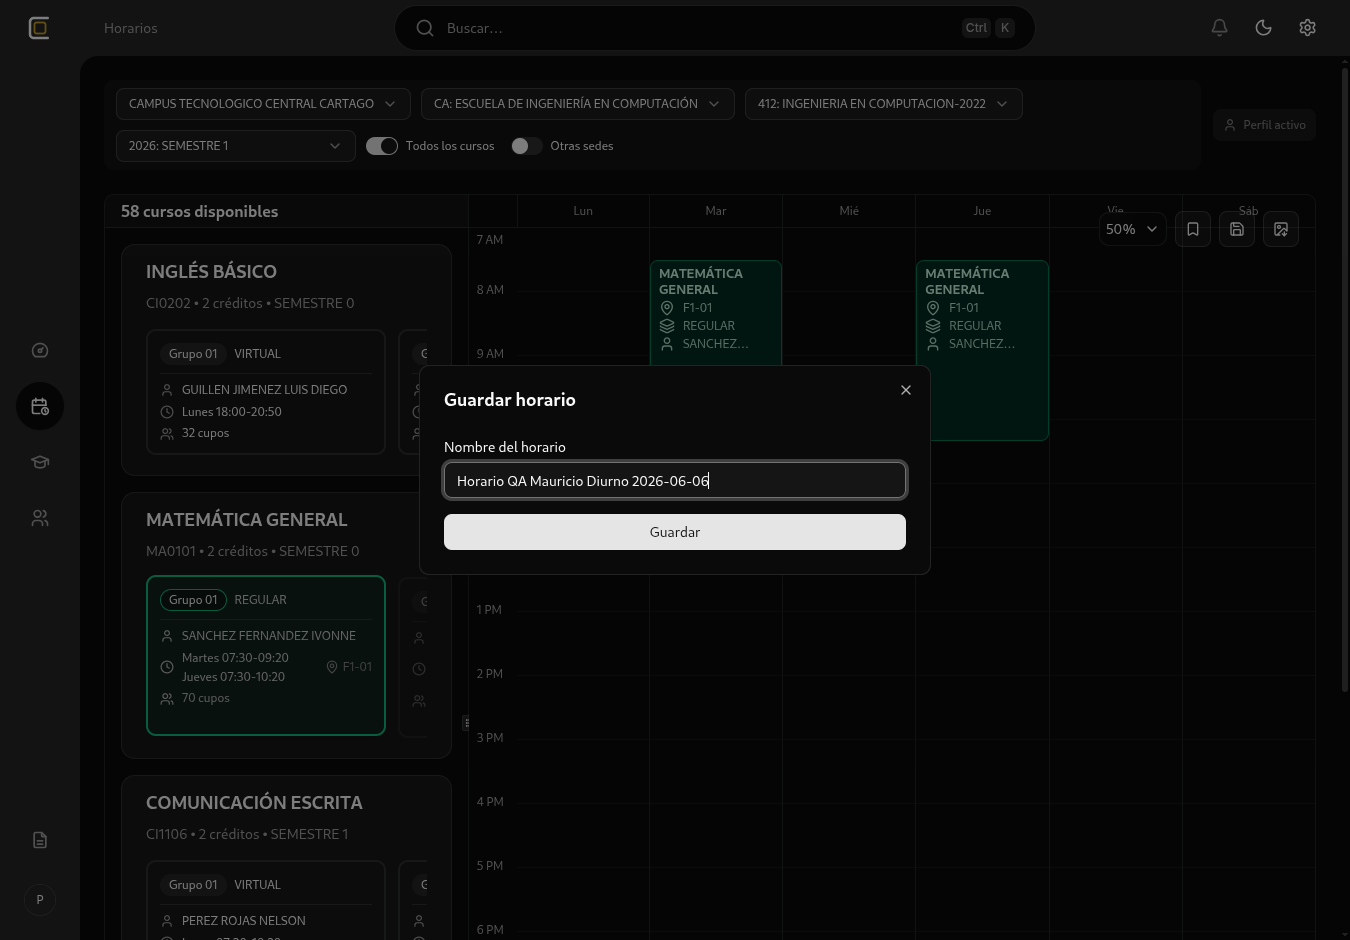
\includegraphics[width=0.92\textwidth]{images/caso-prueba-schedule-guardar-horario.png}
\caption{Registro de horario académico desde el diálogo de guardado}
\label{fig:schedule-guardar}
\end{figure}

\subsubsection{CP-M-004: cargar horario guardado}

El caso CP-M-004 confirmó que el horario guardado aparecía en la lista después de recargar la página, lo cual respalda la persistencia del flujo porque el horario no se pierde al finalizar la interacción inicial.

\begin{figure}[H]
\centering
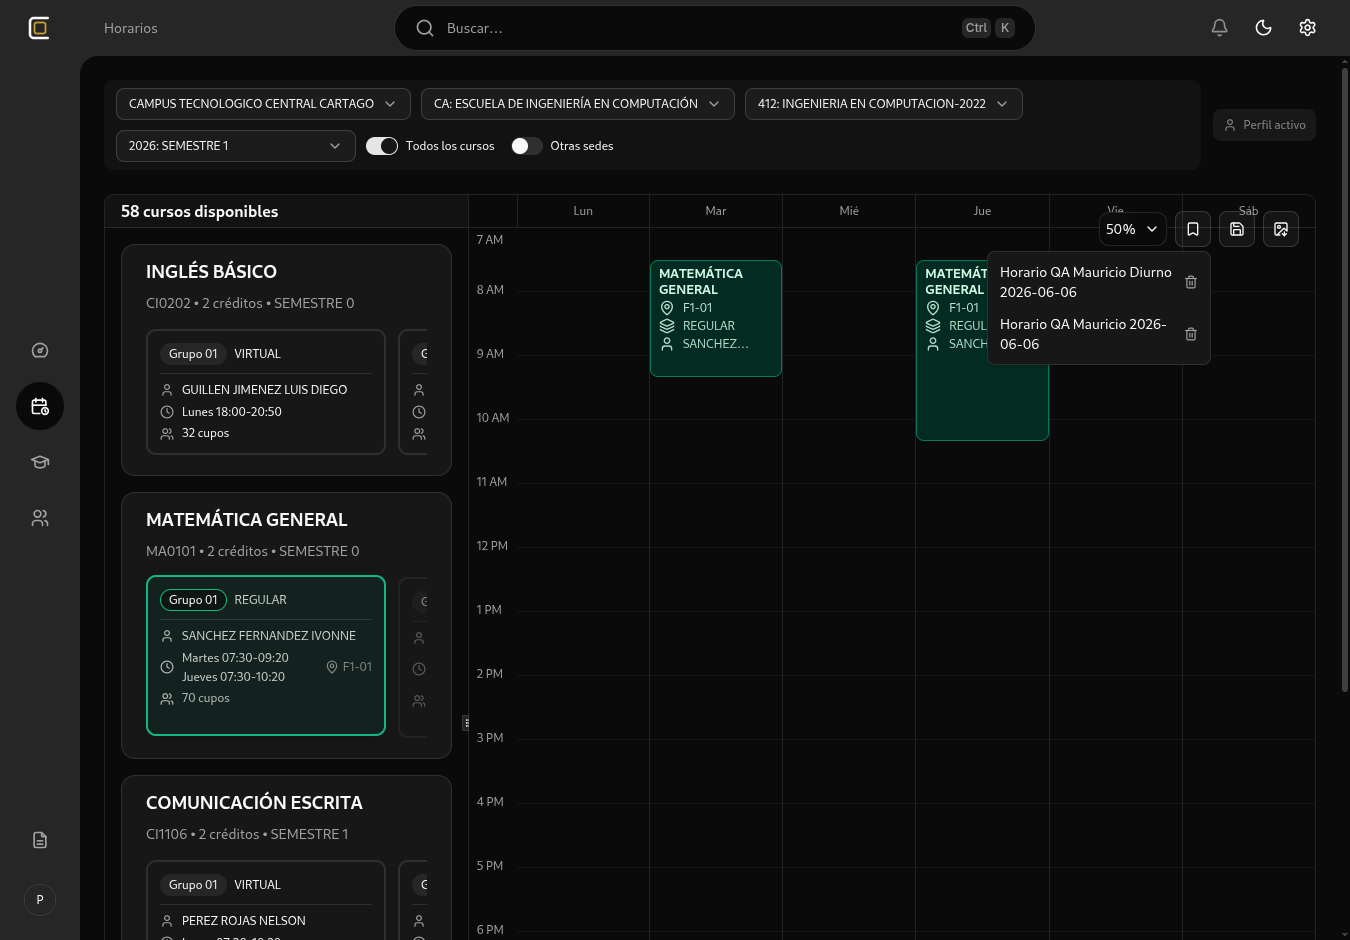
\includegraphics[width=0.92\textwidth]{images/caso-prueba-schedule-cargar-horario.png}
\caption{Disponibilidad del horario guardado para carga posterior}
\label{fig:schedule-cargar}
\end{figure}

\subsubsection{CP-M-006: selección inválida o conflicto de horario}

El caso CP-M-006 abordó un escenario negativo relevante porque, con el grupo \texttt{MA0101-01} seleccionado, la aplicación deshabilitó grupos con traslape los martes o jueves por la mañana, lo que evitó un estado inconsistente. Este comportamiento confirma que la interfaz no solo permite construir horarios, sino que también aplica restricciones preventivas para reducir errores del usuario.

\begin{figure}[H]
\centering
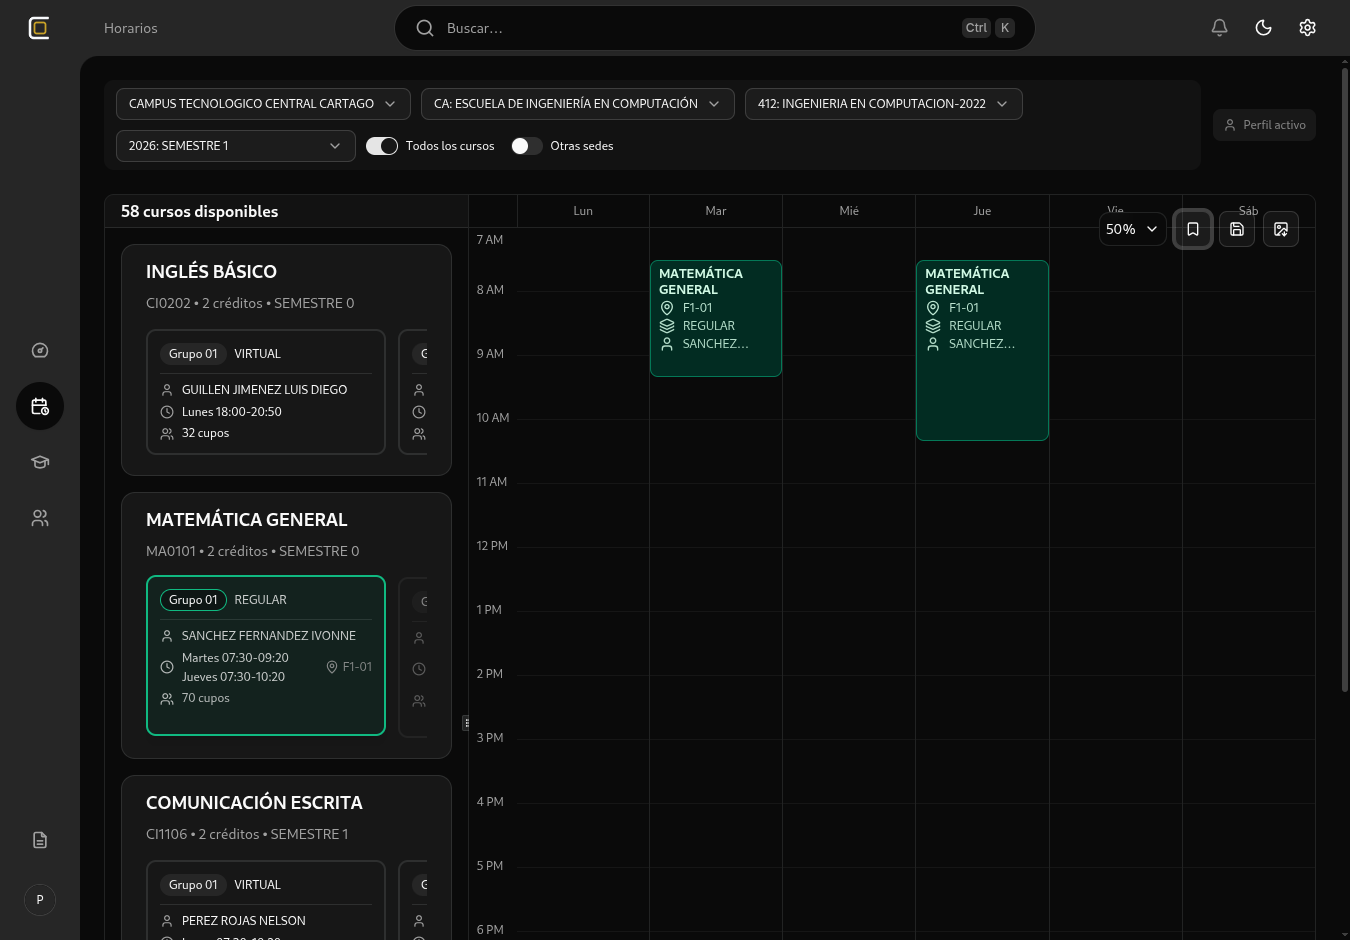
\includegraphics[width=0.92\textwidth]{images/caso-prueba-schedule-conflicto-horario.png}
\caption{Prevención de conflictos mediante deshabilitación de grupos con traslape}
\label{fig:schedule-conflicto}
\end{figure}

\subsubsection{CP-M-005 y CP-M-007: rendimiento y carga ligera en overview}

Para la ruta \texttt{overview}, CP-M-005 midió rendimiento y registró un LCP de 1633 ms con CLS de 0.04, valores que cumplen el umbral definido para RNF-M1 porque el panel cargó en menos de 2 segundos. Además, Lighthouse registró accesibilidad 100, buenas prácticas 100 y SEO 66, mientras que CP-M-007 complementó esta medición con una prueba de carga ligera de 30 solicitudes, concurrencia 3, cero solicitudes fallidas, 7.46 solicitudes por segundo y tiempo medio total de 402.189 ms por solicitud.

\begin{figure}[H]
\centering
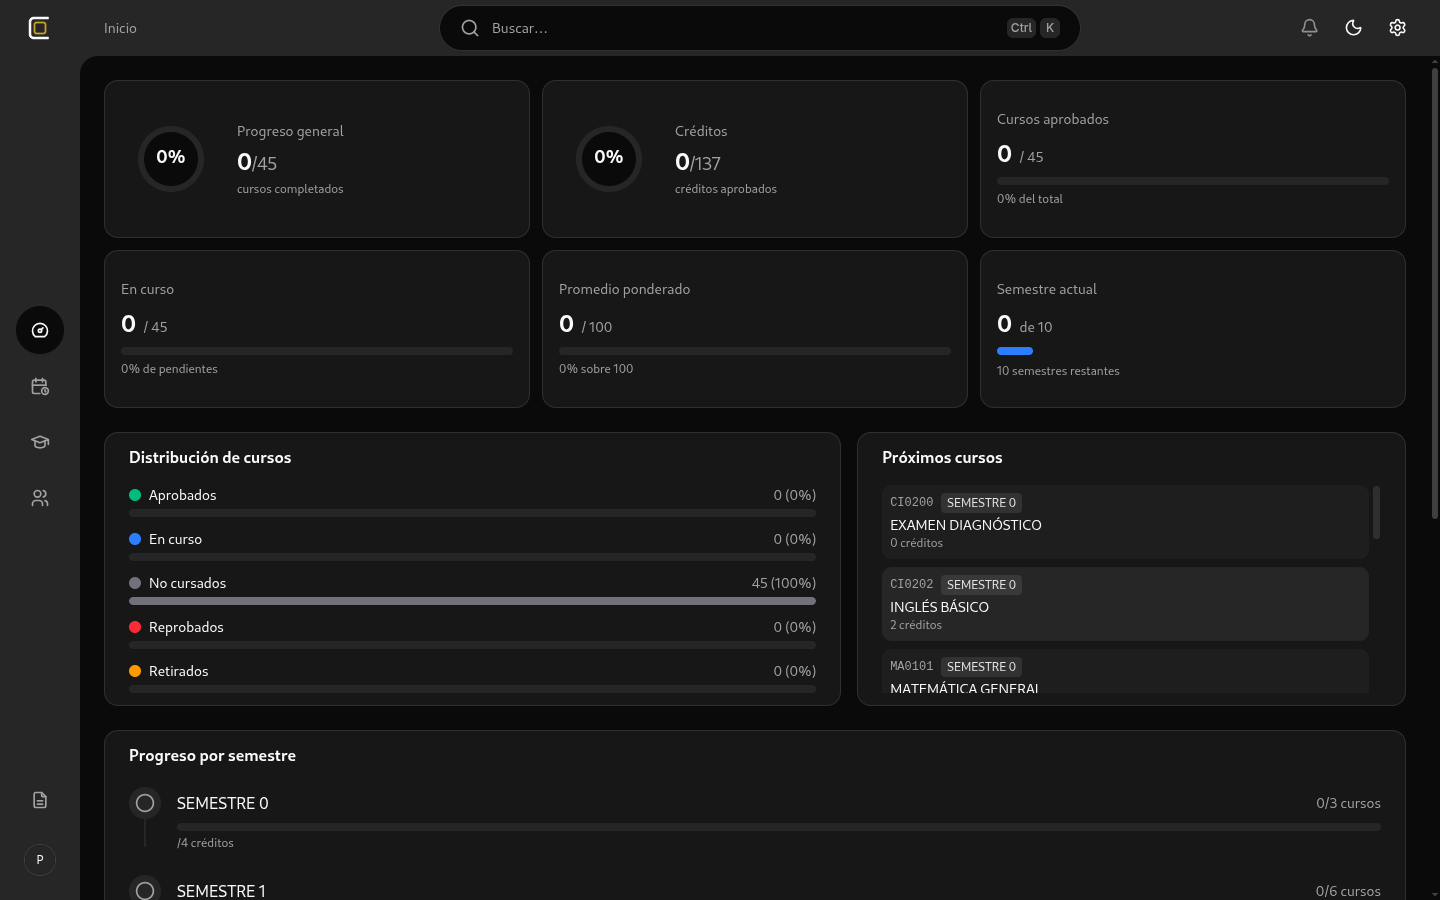
\includegraphics[width=0.92\textwidth]{images/resultado-overview-panel-resumen.png}
\caption{Panel de resumen utilizado para la evaluación de rendimiento de \texttt{overview}}
\label{fig:overview-rendimiento}
\end{figure}

\subsubsection{CP-M-008 y CP-M-009: lógica de horarios y aceptación de usuario}

El caso CP-M-008 ejecutó 4 pruebas unitarias sobre utilidades de calendario con resultado aprobado y, como cierre del módulo, CP-M-009 confirmó la aceptación del flujo principal de creación y reutilización de horarios mediante Playwright, integrando acceso, selección de grupo, guardado y verificación de disponibilidad posterior.

\begin{figure}[H]
\centering
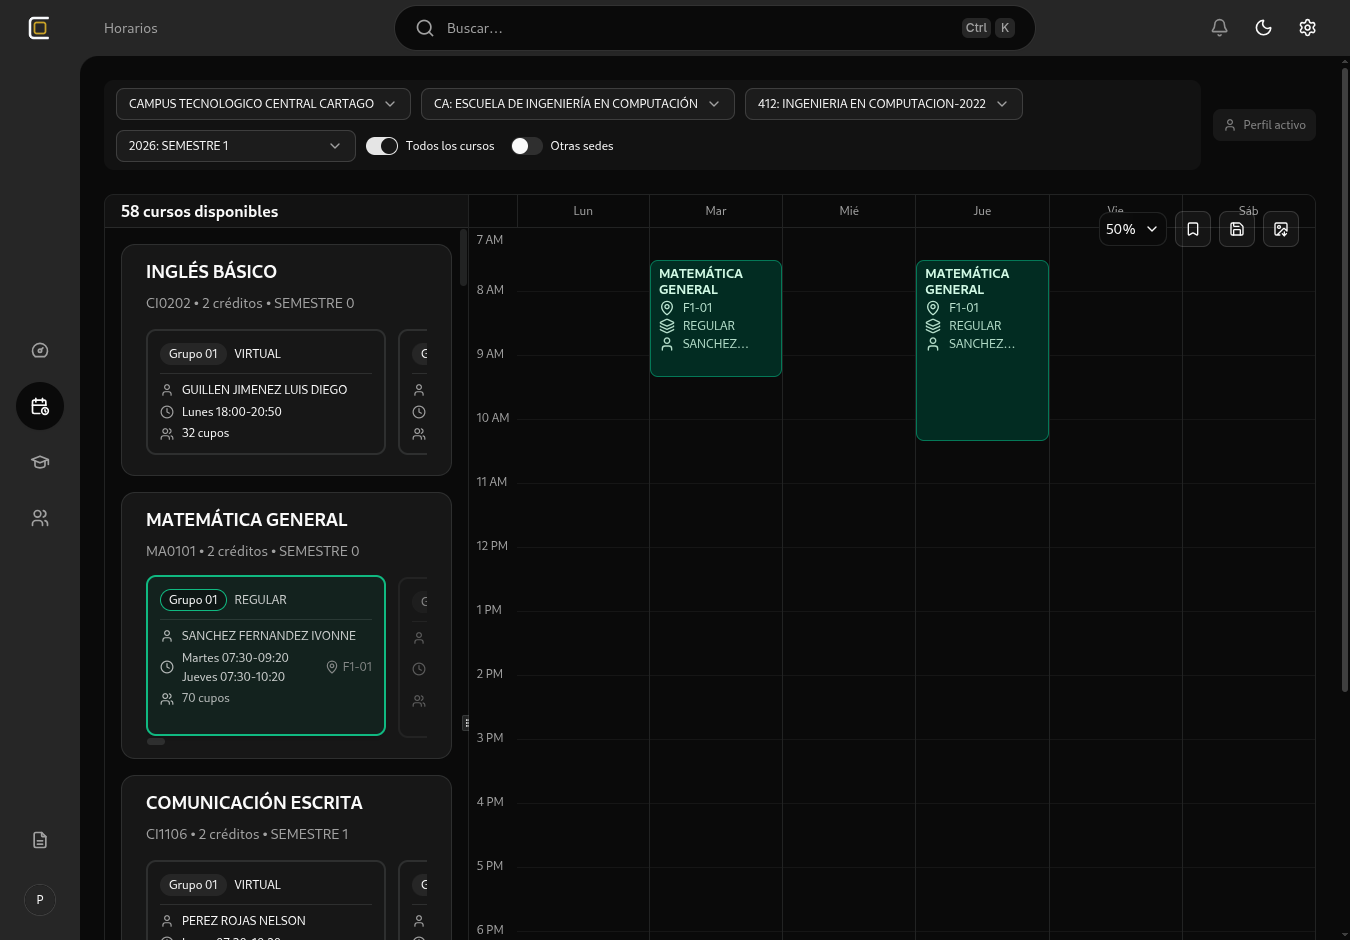
\includegraphics[width=0.92\textwidth]{images/aceptacion-usuario-creador-horarios.png}
\caption{Evidencia de aceptación de usuario del flujo de creación de horarios}
\label{fig:schedule-uat}
\end{figure}

\subsection{Ruta professors y API de reseñas}

El módulo de profesores fue evaluado desde la búsqueda y consulta hasta la validación del formulario de reseñas, la seguridad de entradas y la automatización de API, por lo que cada evidencia se presenta junto al caso que respalda.

\subsubsection{CP-I-001: buscar profesor}

CP-I-001 confirmó el acceso al detalle del profesor \texttt{CORDERO QUIROS MARCIAL} en la ruta \texttt{/professors/480}, donde se observaron métricas generales, etiquetas destacadas y la sección de reseñas del profesor consultado.

\begin{figure}[H]
\centering
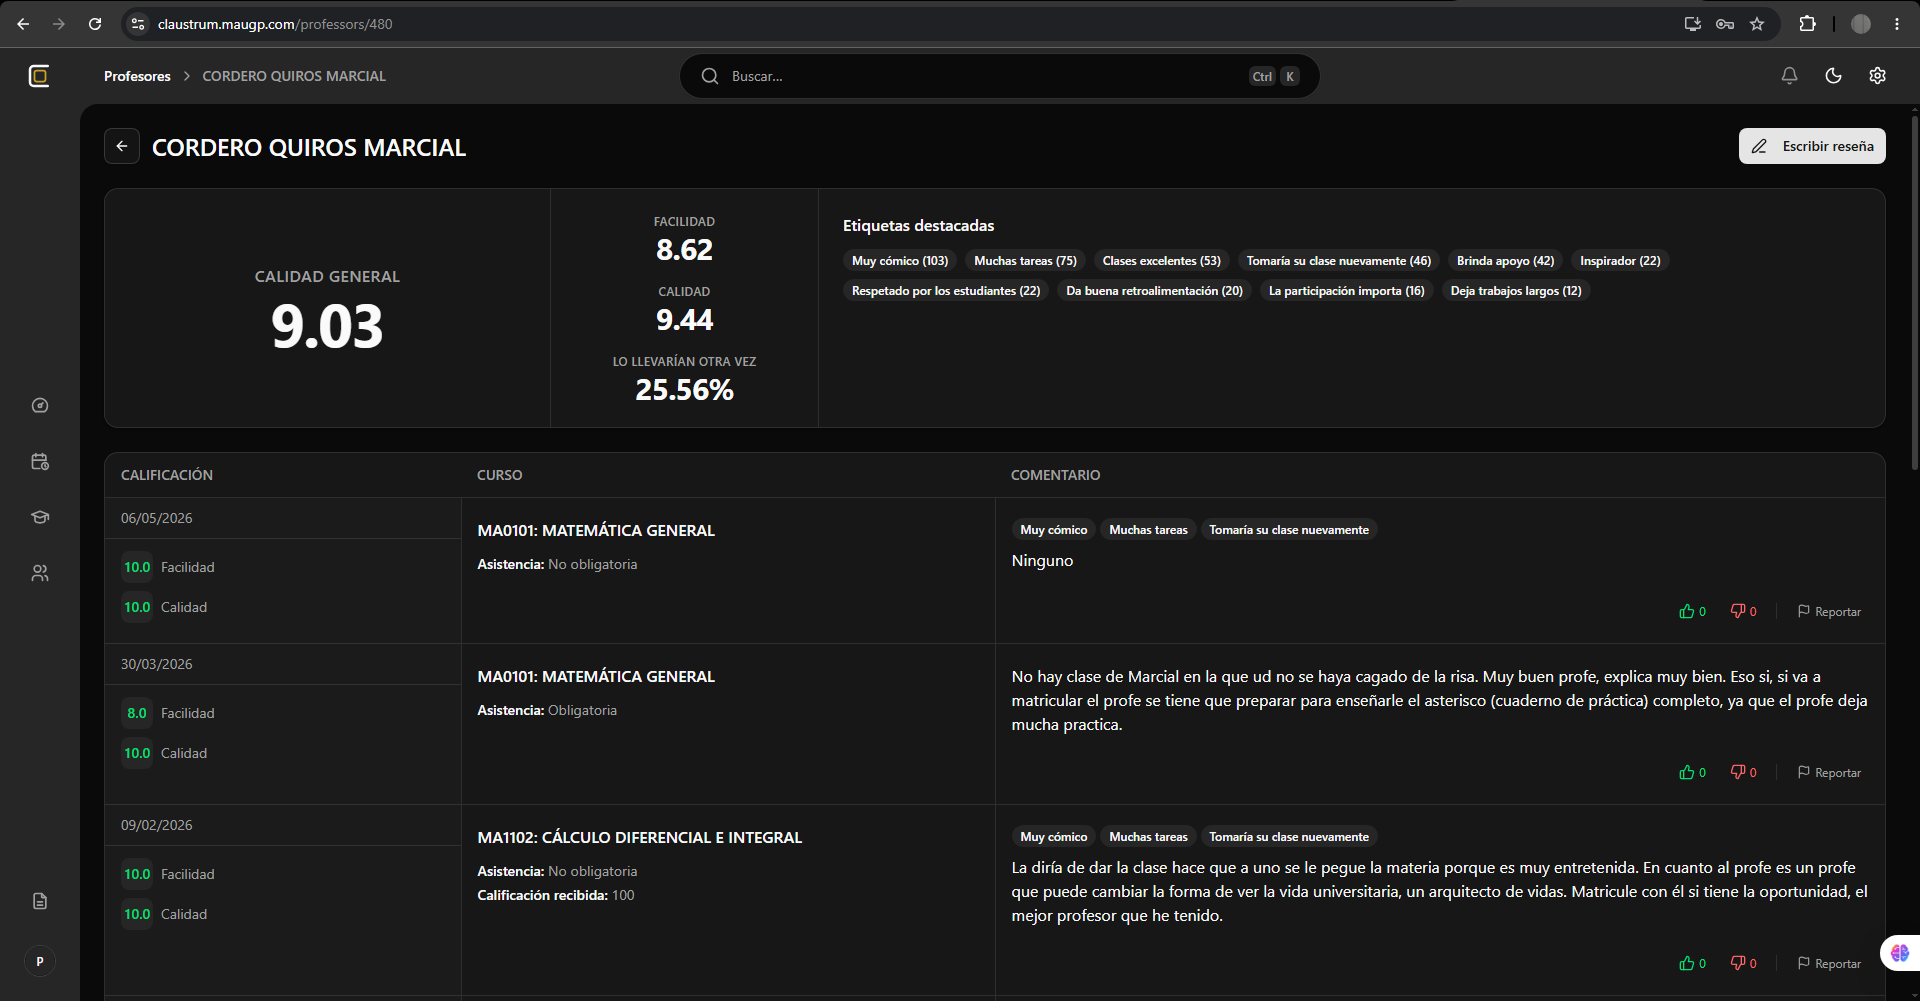
\includegraphics[width=0.92\textwidth]{images/caso-prueba-professors-buscar-profesor.png}
\caption{Consulta del detalle de profesor desde la ruta \texttt{professors}}
\label{fig:professors-busqueda}
\end{figure}

\subsubsection{CP-I-002: consultar reseñas existentes}

CP-I-002 verificó que las reseñas existentes mostraran fecha, curso asociado, calificaciones, etiquetas, comentario y opciones de interacción, de manera que la evidencia permite comprobar que el módulo no se limita a mostrar una ficha de profesor, sino que también presenta información evaluativa previamente registrada.

\begin{figure}[H]
\centering
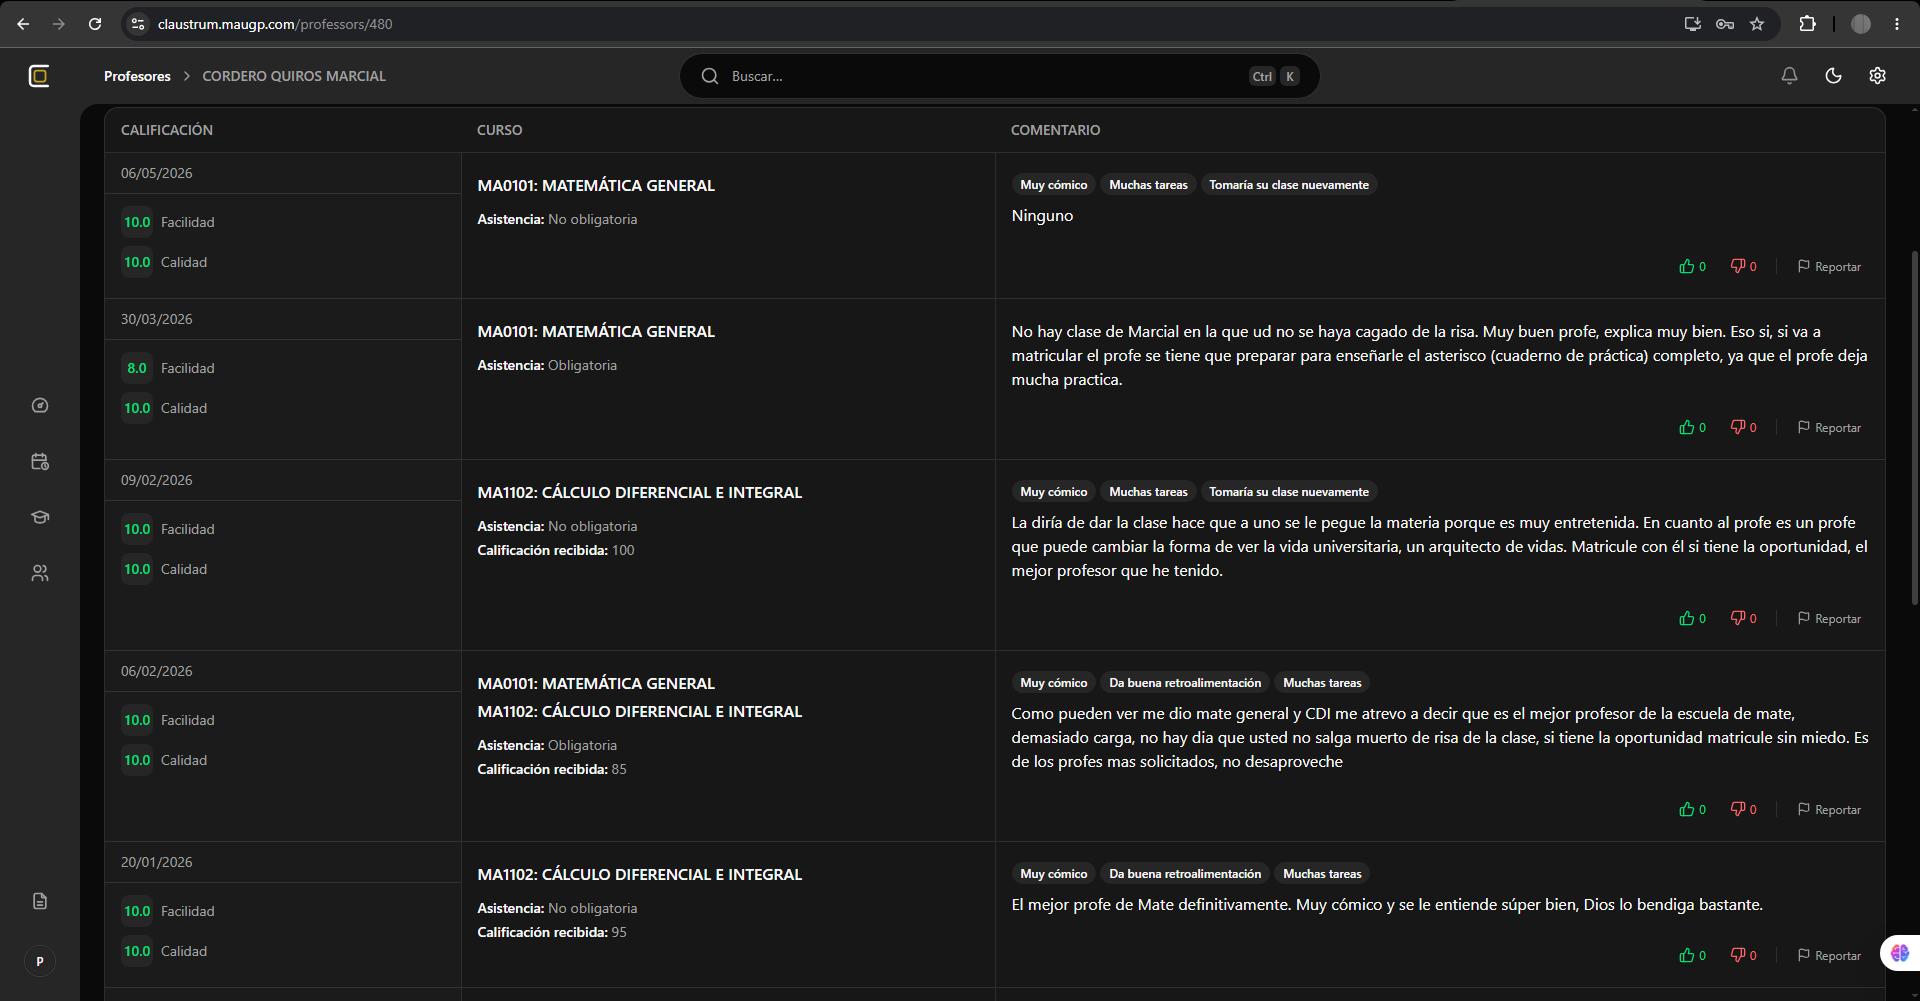
\includegraphics[width=0.92\textwidth]{images/caso-prueba-professors-consultar-resenas.png}
\caption{Visualización de reseñas existentes asociadas al profesor consultado}
\label{fig:professors-resenas}
\end{figure}

\subsubsection{CP-I-003: enviar reseña válida}

El caso CP-I-003 produjo el hallazgo más relevante del proyecto, ya que al completar el formulario con una reseña aparentemente válida, incluyendo curso, calificación obtenida, comentario, calificaciones numéricas, asistencia obligatoria y etiqueta, la aplicación rechazó el envío con el mensaje \texttt{Invalid review payload}. Este resultado fallido impide completar el requisito funcional RF-I1 porque el usuario puede consultar reseñas, pero no logra enviar una reseña válida, como se evidencia en la figura \ref{fig:defecto-resena-valida}.

\begin{figure}[H]
\centering
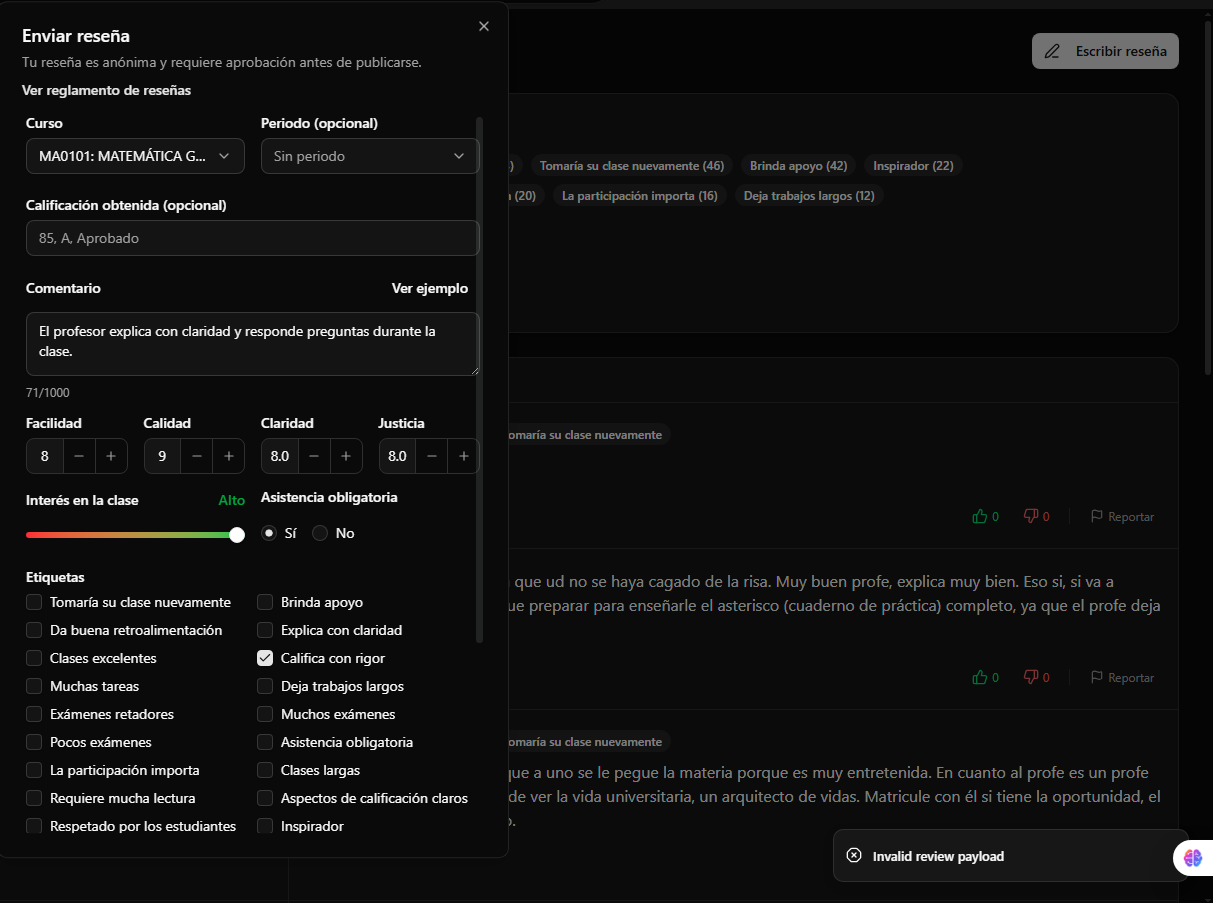
\includegraphics[width=0.92\textwidth]{images/defecto-professors-rechazo-resena-valida.png}
\caption{Rechazo de una reseña válida mediante el mensaje \texttt{Invalid review payload}}
\label{fig:defecto-resena-valida}
\end{figure}

\subsubsection{CP-I-004: campos obligatorios vacíos}

CP-I-004 validó que los campos obligatorios vacíos fueran rechazados con el mensaje \texttt{Revisa los datos del formulario y vuelve a intentar}, lo cual demuestra que el formulario cuenta con validaciones mínimas para evitar envíos incompletos.

\begin{figure}[H]
\centering
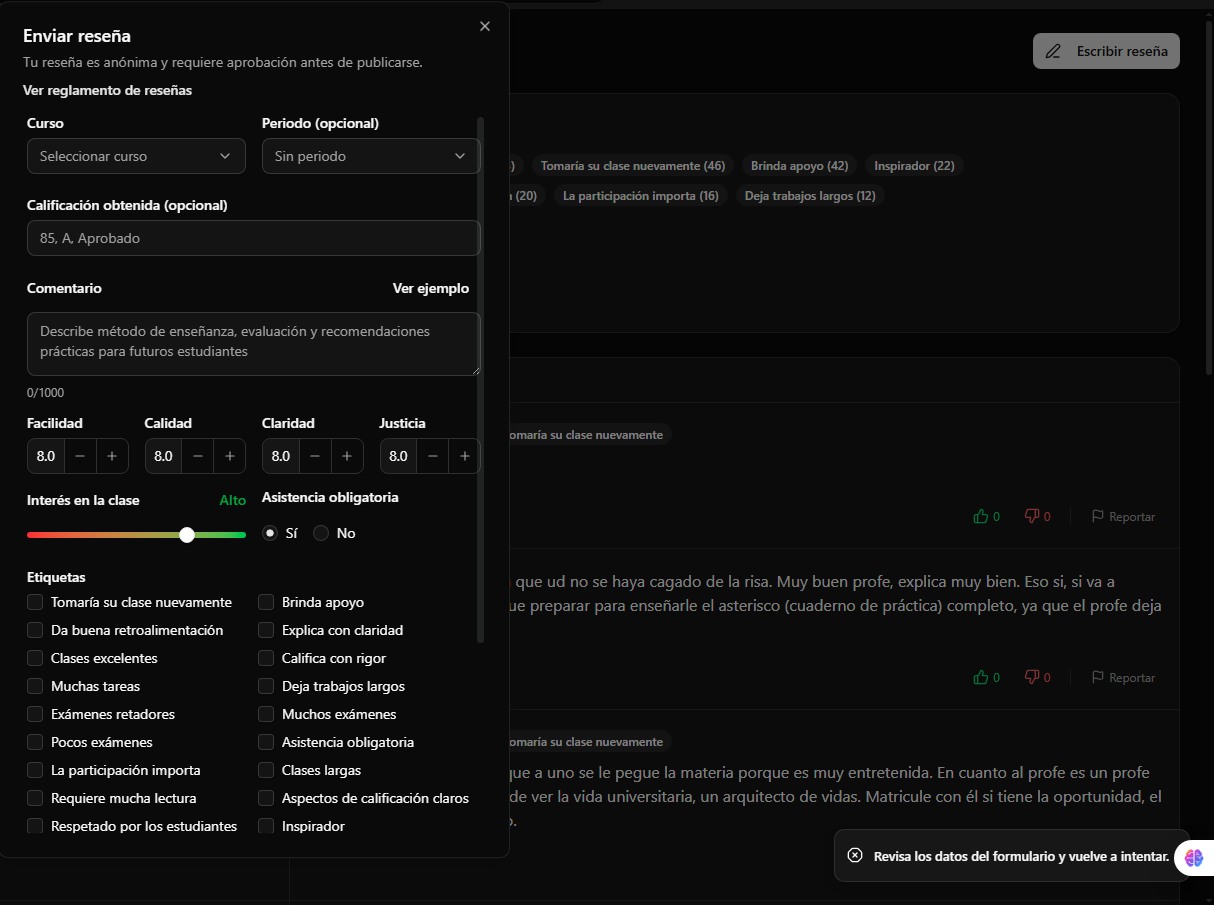
\includegraphics[width=0.92\textwidth]{images/caso-prueba-professors-campos-obligatorios.png}
\caption{Validación de campos obligatorios vacíos en el formulario de reseñas}
\label{fig:professors-campos}
\end{figure}

\subsubsection{CP-I-005: intento de XSS}

CP-I-005 ingresó el payload \texttt{<script>alert('xss')</script>} y observó rechazo sin ejecución de script ni aparición de alerta, por lo que el resultado respalda el requisito RNF-I1 en el escenario de entrada maliciosa evaluado desde el formulario de reseñas.

\begin{figure}[H]
\centering
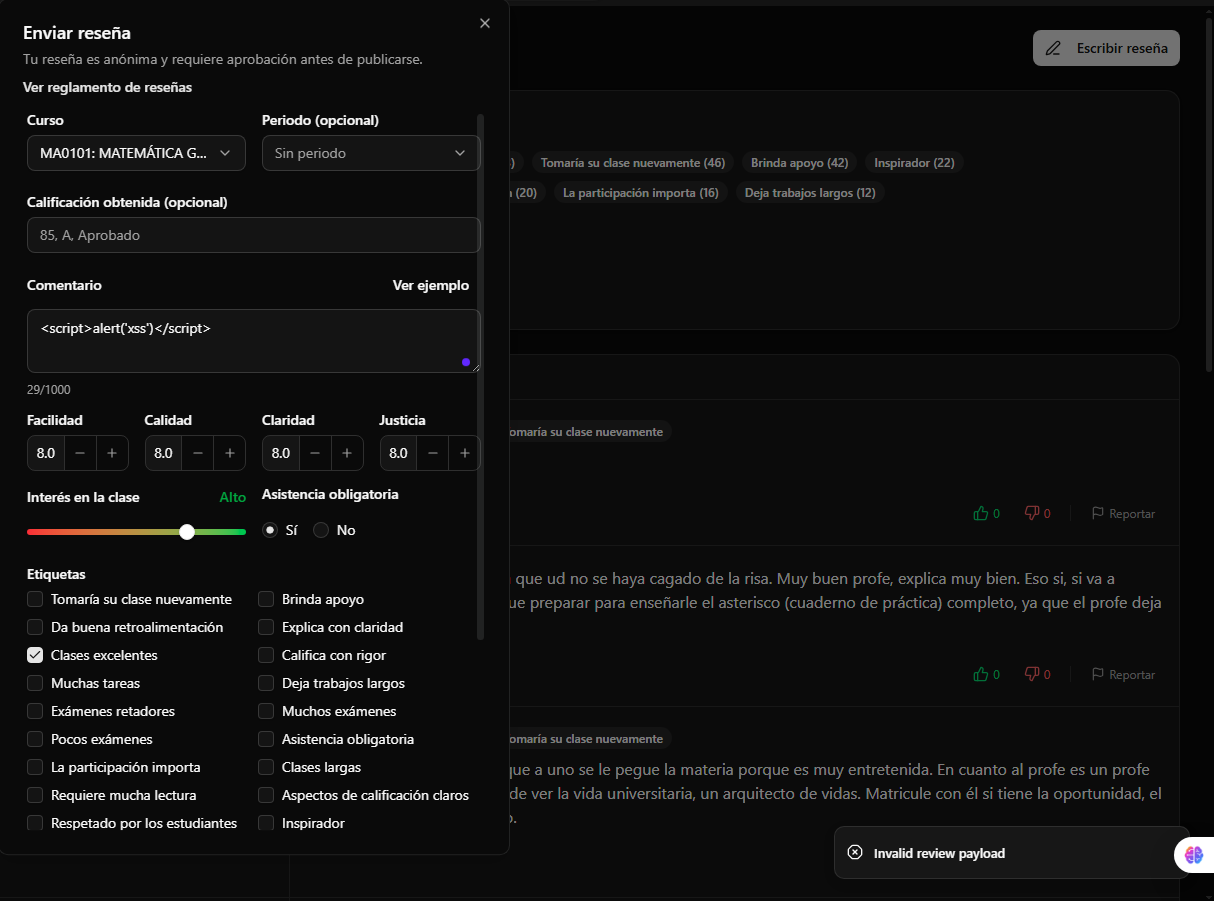
\includegraphics[width=0.92\textwidth]{images/caso-prueba-professors-validacion-xss.png}
\caption{Rechazo de entrada XSS sin ejecución de código en el navegador}
\label{fig:professors-xss}
\end{figure}

\subsubsection{CP-I-008: intento de SQL Injection}

CP-I-008 utilizó el payload \texttt{' OR '1'='1} en el buscador y la aplicación trató la entrada como texto, sin que se observaran errores SQL, exposición de datos no autorizados ni comportamiento anómalo de consulta.

\begin{figure}[H]
\centering
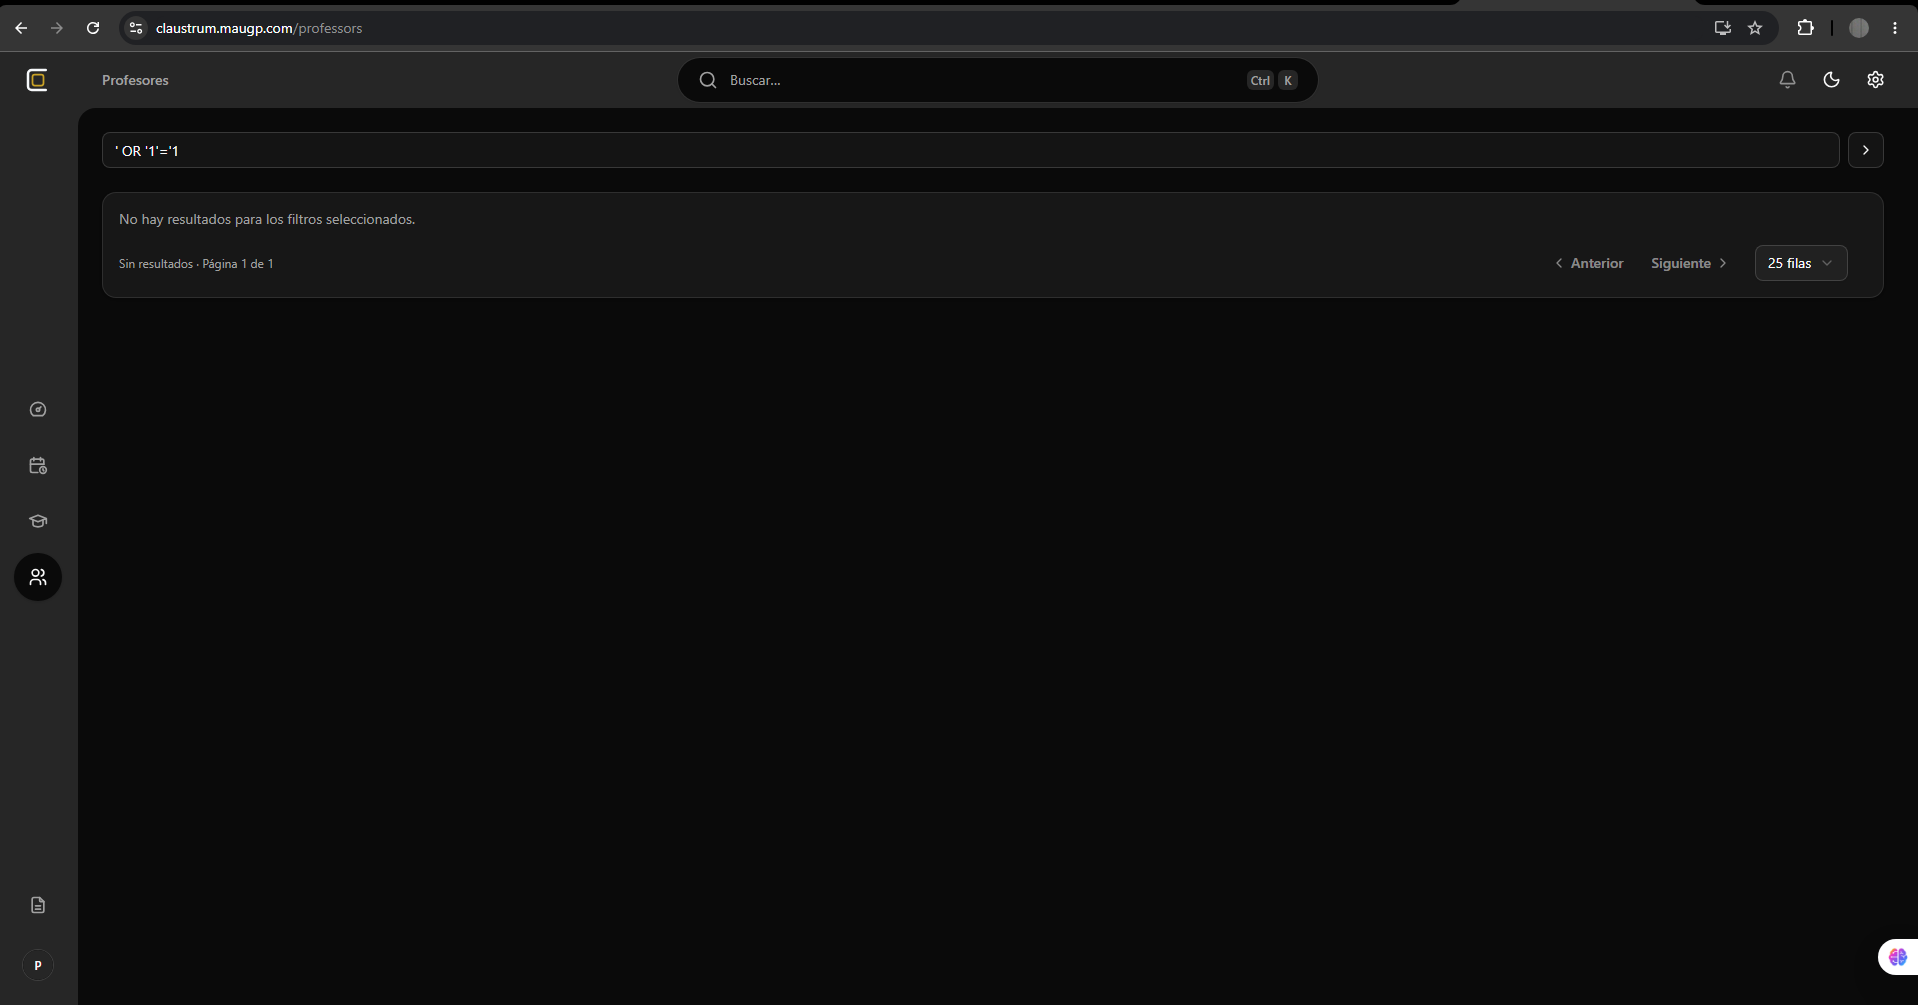
\includegraphics[width=0.92\textwidth]{images/caso-prueba-professors-sql-injection.png}
\caption{Tratamiento seguro de una entrada tipo SQL Injection en búsqueda de profesores}
\label{fig:professors-sql}
\end{figure}

\subsubsection{CP-I-006: API de reseñas}

CP-I-006 evaluó la API mediante Newman, con una colección que ejecutó 4 solicitudes contra endpoints reales de Supabase RPC y cubrió resumen de reseñas, consulta de reseñas públicas aprobadas, una entrada tipo SQL Injection y una entrada tipo XSS. Todas las solicitudes respondieron 200 OK, se ejecutaron 14 aserciones y no se registraron fallos, aunque este resultado favorable en API no invalida el defecto funcional observado en la interfaz, ya que el fallo de envío se presentó en el flujo de usuario.

\subsubsection{CP-I-007: aceptación de usuario del flujo de reseñas}

CP-I-007 comprobó que el usuario puede abrir la ruta de profesores, consultar el detalle, identificar reseñas existentes y acceder al formulario mediante la opción de escribir reseña. No obstante, el flujo de aceptación no se completó debido al rechazo de la reseña válida, por lo que el caso quedó fallido y vinculado con DEF-I-001.

\begin{figure}[H]
\centering
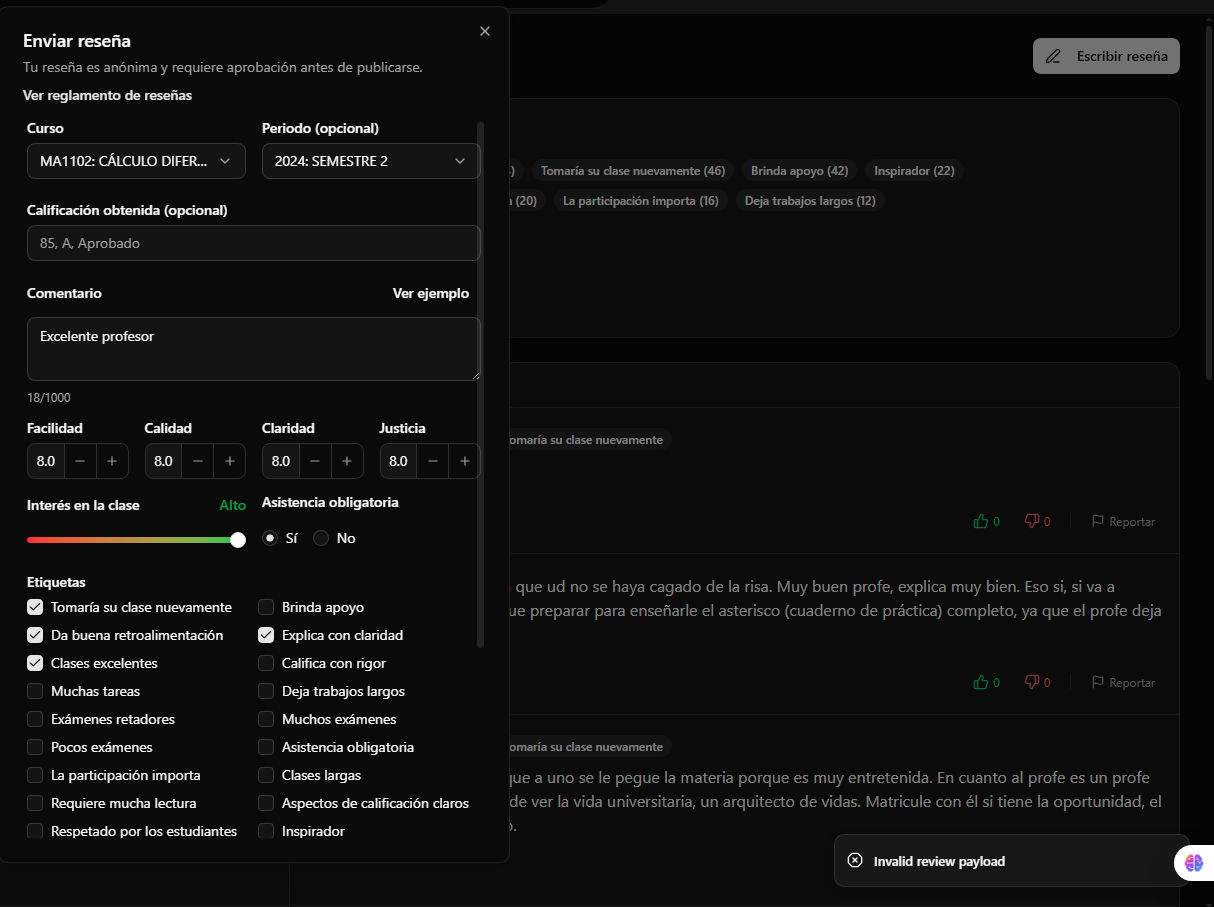
\includegraphics[width=0.92\textwidth]{images/aceptacion-usuario-professors-resenas.png}
\caption{Evidencia de aceptación de usuario del flujo de consulta y envío de reseñas}
\label{fig:professors-uat}
\end{figure}

La automatización con Playwright respaldó la navegación hasta el formulario de reseña, y esta evidencia complementa el caso de aceptación porque demuestra que el flujo puede alcanzar la pantalla de captura de datos, aunque el envío final falle por la validación reportada.

\begin{figure}[H]
\centering
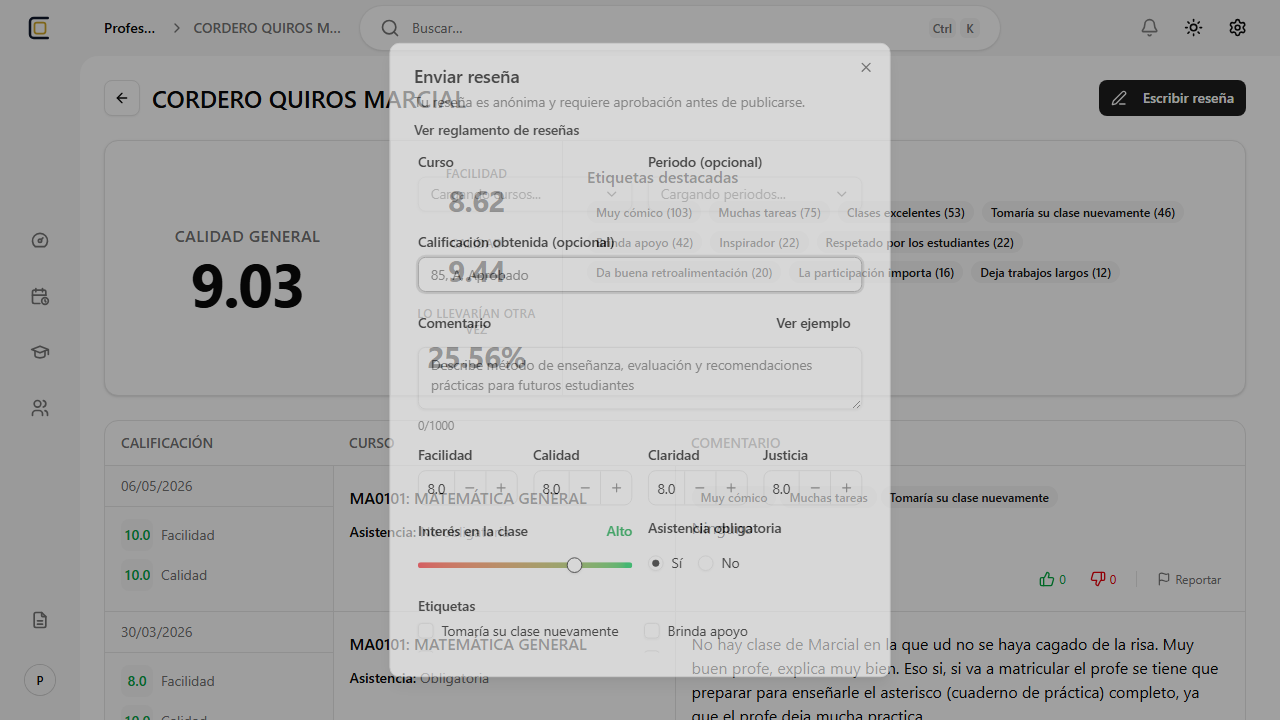
\includegraphics[width=0.92\textwidth]{images/automatizacion-professors-formulario-resena.png}
\caption{Apertura automatizada del formulario de reseña mediante Playwright}
\label{fig:professors-playwright}
\end{figure}

\subsection{Rutas auth, onboarding y curriculum}

Las rutas \texttt{auth}, \texttt{onboarding} y \texttt{curriculum} fueron revisadas para validar acceso, redirección académica, navegación y consulta de información curricular, con la evidencia presentada según el orden de los casos ejecutados.

\subsubsection{CP-A-001: login válido}

CP-A-001 confirmó que el usuario demo puede iniciar sesión correctamente y acceder a la aplicación autenticada, por lo que esta prueba respalda el flujo positivo de autenticación y permite continuar con los demás escenarios protegidos.

\begin{figure}[H]
\centering
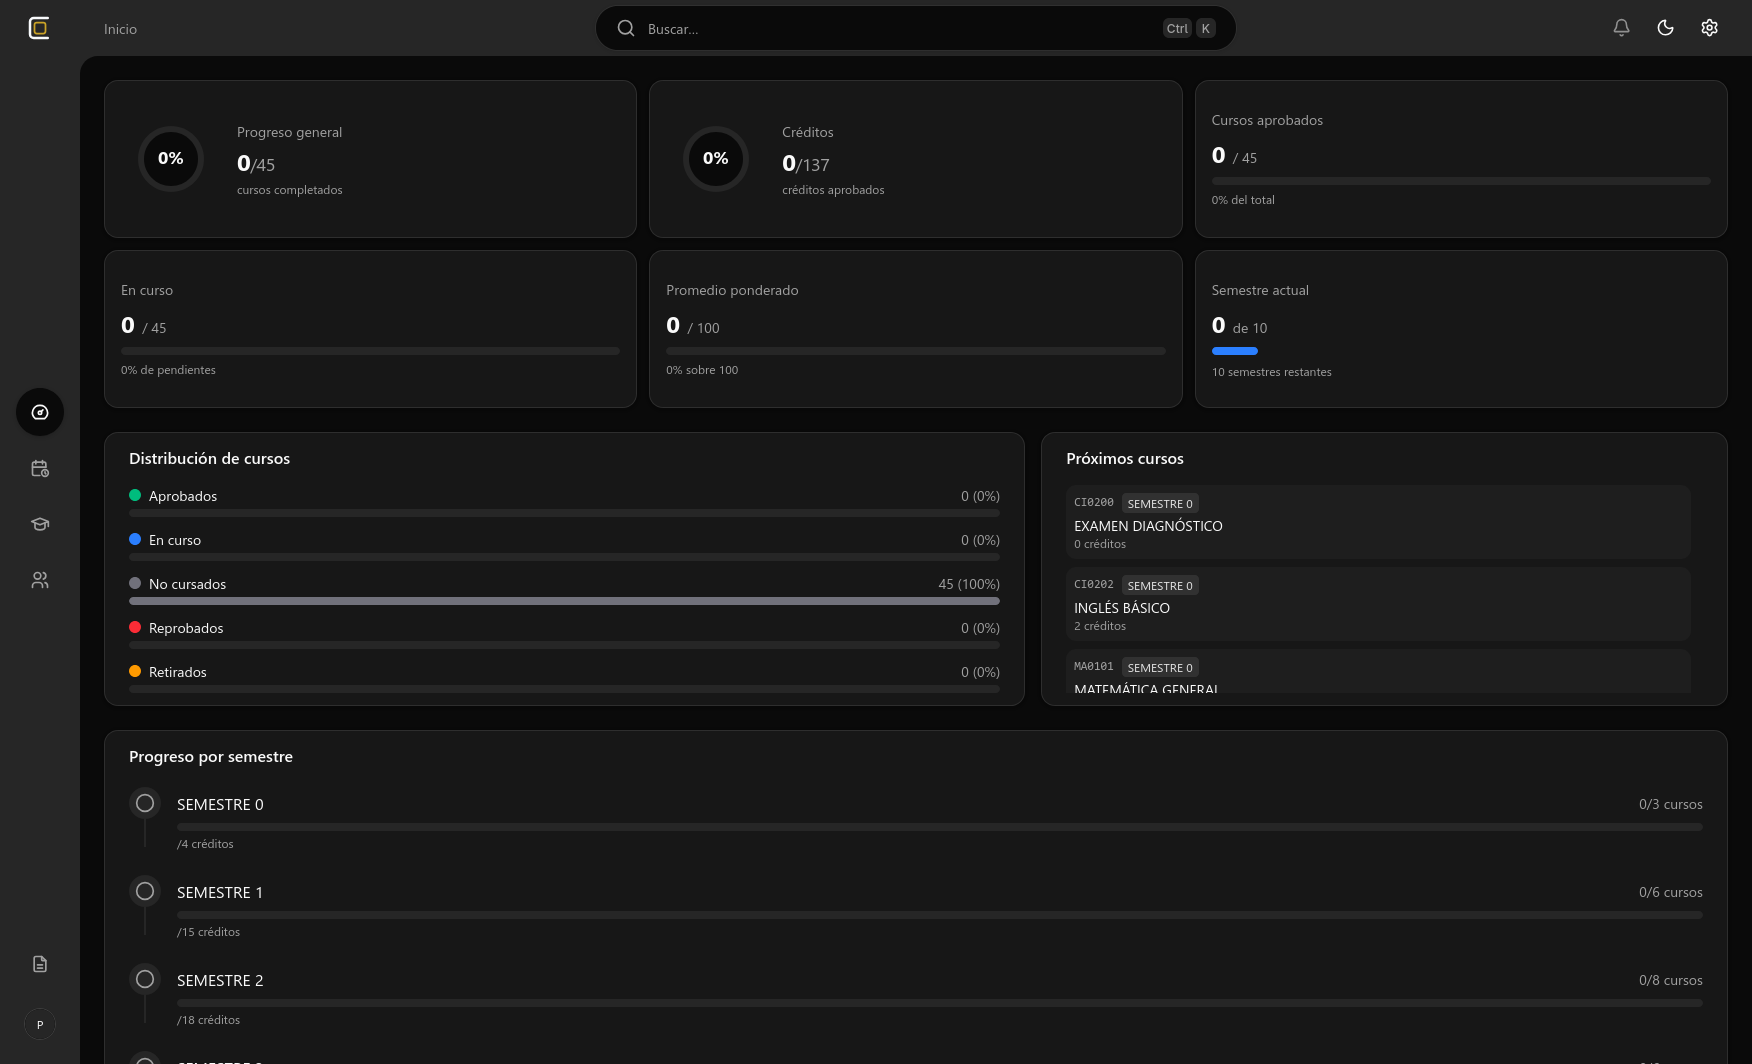
\includegraphics[width=0.92\textwidth]{images/caso-prueba-auth-login-valido.png}
\caption{Inicio de sesión exitoso con credenciales válidas}
\label{fig:auth-login-valido}
\end{figure}

\subsubsection{CP-A-002: login inválido}

CP-A-002 identificó un defecto de mensajería, ya que al ingresar un correo con formato correcto y una contraseña incorrecta la aplicación mostró un mensaje sobre formato inválido de correo electrónico. Aunque este problema no bloquea el control de acceso, sí afecta claridad y precisión de la retroalimentación al usuario.

\begin{figure}[H]
\centering
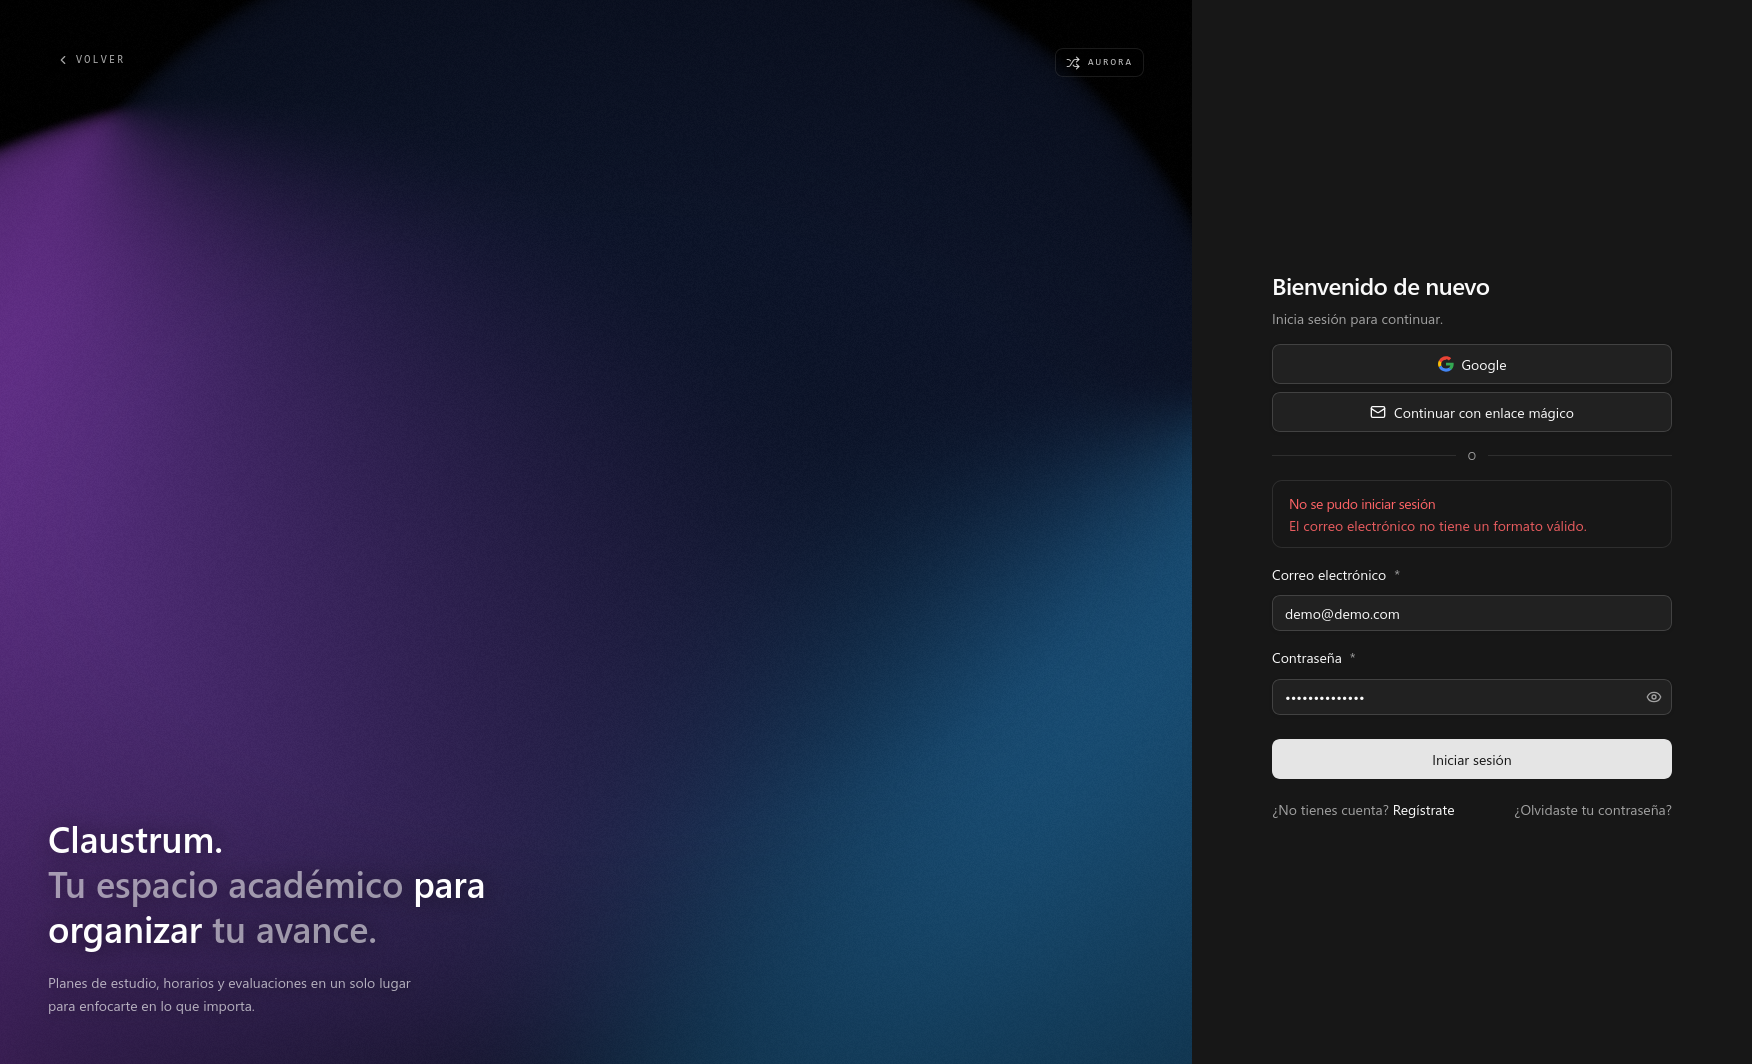
\includegraphics[width=0.92\textwidth]{images/defecto-auth-mensaje-login-invalido.png}
\caption{Mensaje incorrecto presentado durante el intento de inicio de sesión inválido}
\label{fig:defecto-login-invalido}
\end{figure}

\subsubsection{CP-A-003: onboarding académico}

CP-A-003 verificó el onboarding académico del usuario \texttt{demo@demo.com}, quien ya tenía completado el proceso, por lo que se validó la redirección correcta hacia la aplicación. Este resultado confirma que el sistema maneja adecuadamente el estado académico inicial del usuario probado.

\begin{figure}[H]
\centering
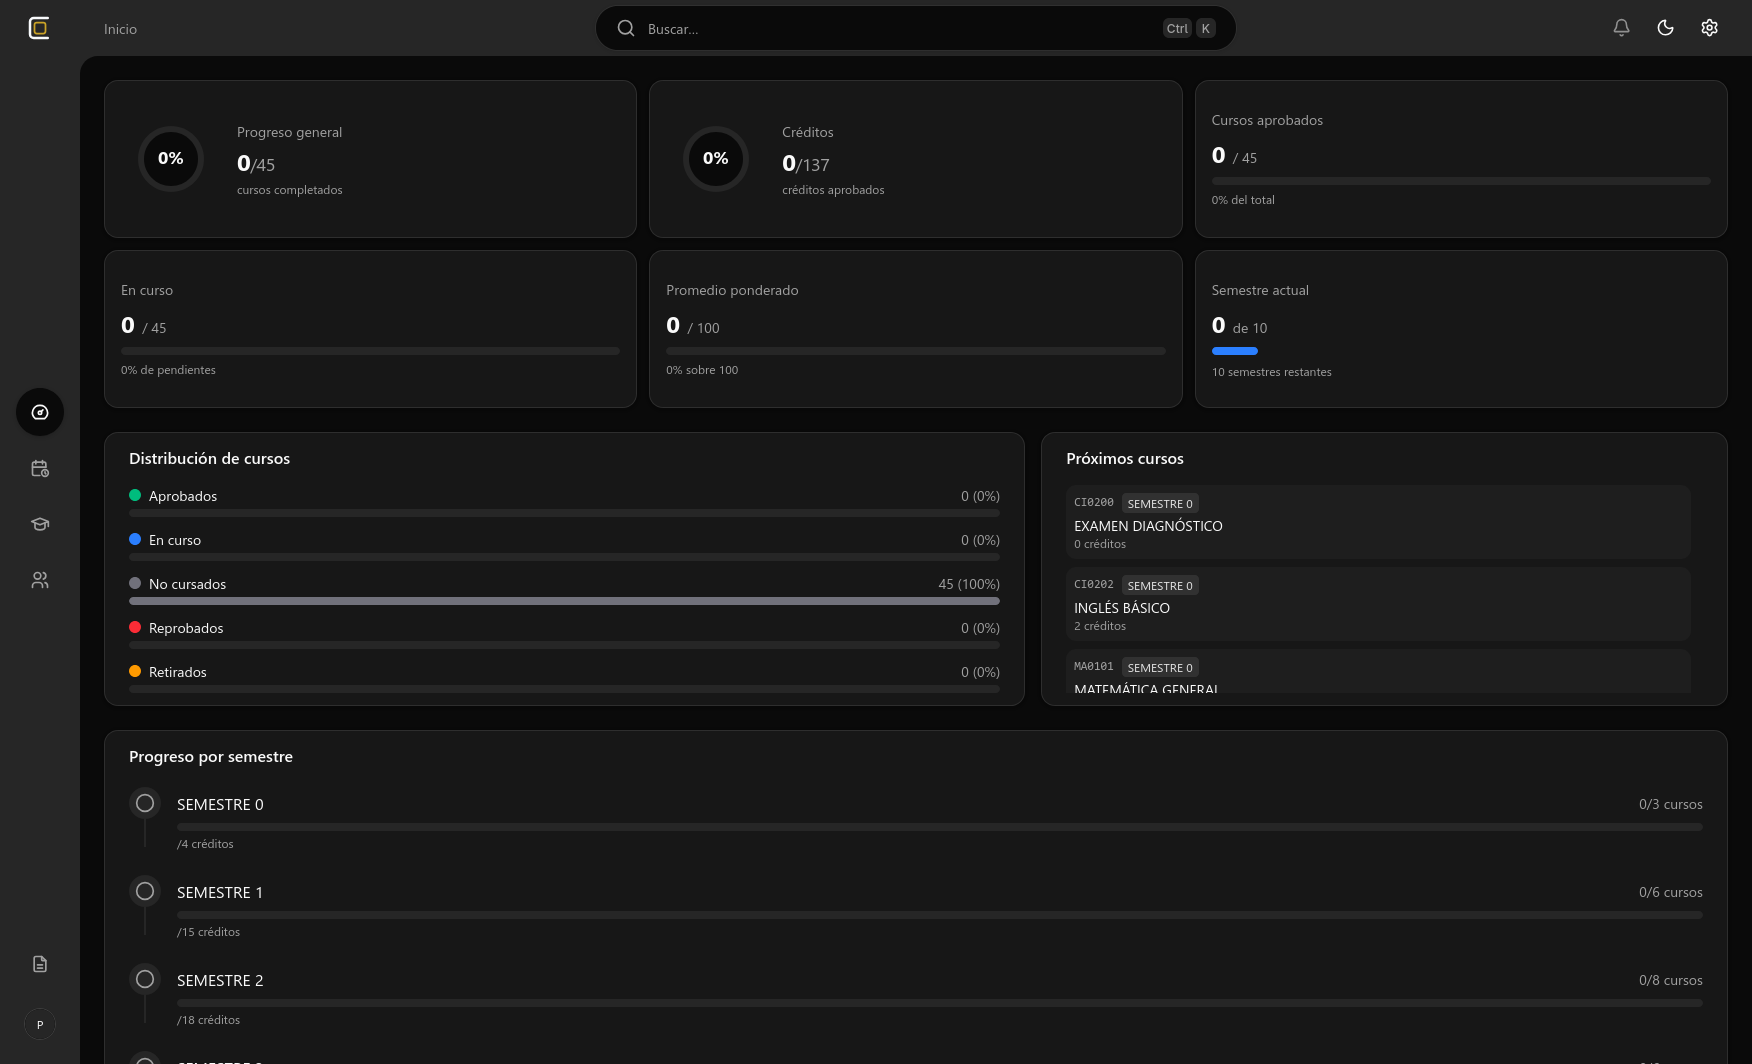
\includegraphics[width=0.92\textwidth]{images/caso-prueba-onboarding-redireccion.png}
\caption{Redirección correcta de usuario con onboarding académico completado}
\label{fig:onboarding}
\end{figure}

\subsubsection{CP-A-008: control de acceso sin sesión}

CP-A-008 evaluó control de acceso sin sesión activa en rutas protegidas y observó bloqueos correctos en \texttt{/settings} y en el inicio, con lo cual respalda el requisito RF-A1 desde la perspectiva de seguridad básica porque evita acceso directo a contenido protegido.

\begin{figure}[H]
\centering
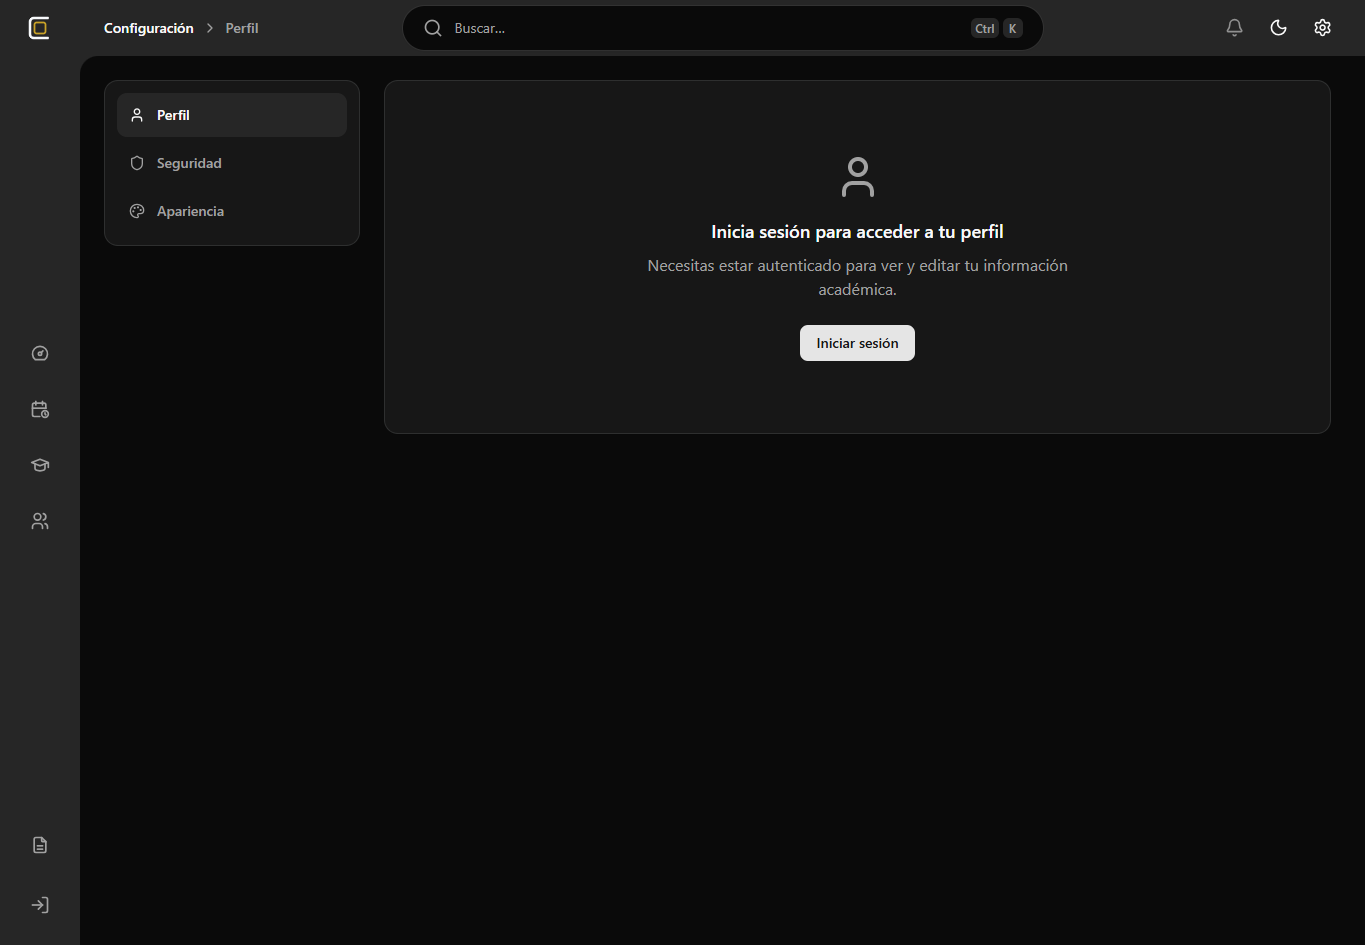
\includegraphics[width=0.92\textwidth]{images/caso-prueba-auth-control-acceso.png}
\caption{Bloqueo de acceso a rutas protegidas sin sesión válida}
\label{fig:control-acceso}
\end{figure}

\subsubsection{CP-A-004: detalle de curso en la malla curricular}

CP-A-004 confirmó que los cursos muestran créditos, horas y semestre correspondiente, de modo que esta evidencia respalda la utilidad de la ruta \texttt{curriculum}, ya que el usuario puede consultar información académica concreta desde la malla curricular.

\begin{figure}[H]
\centering
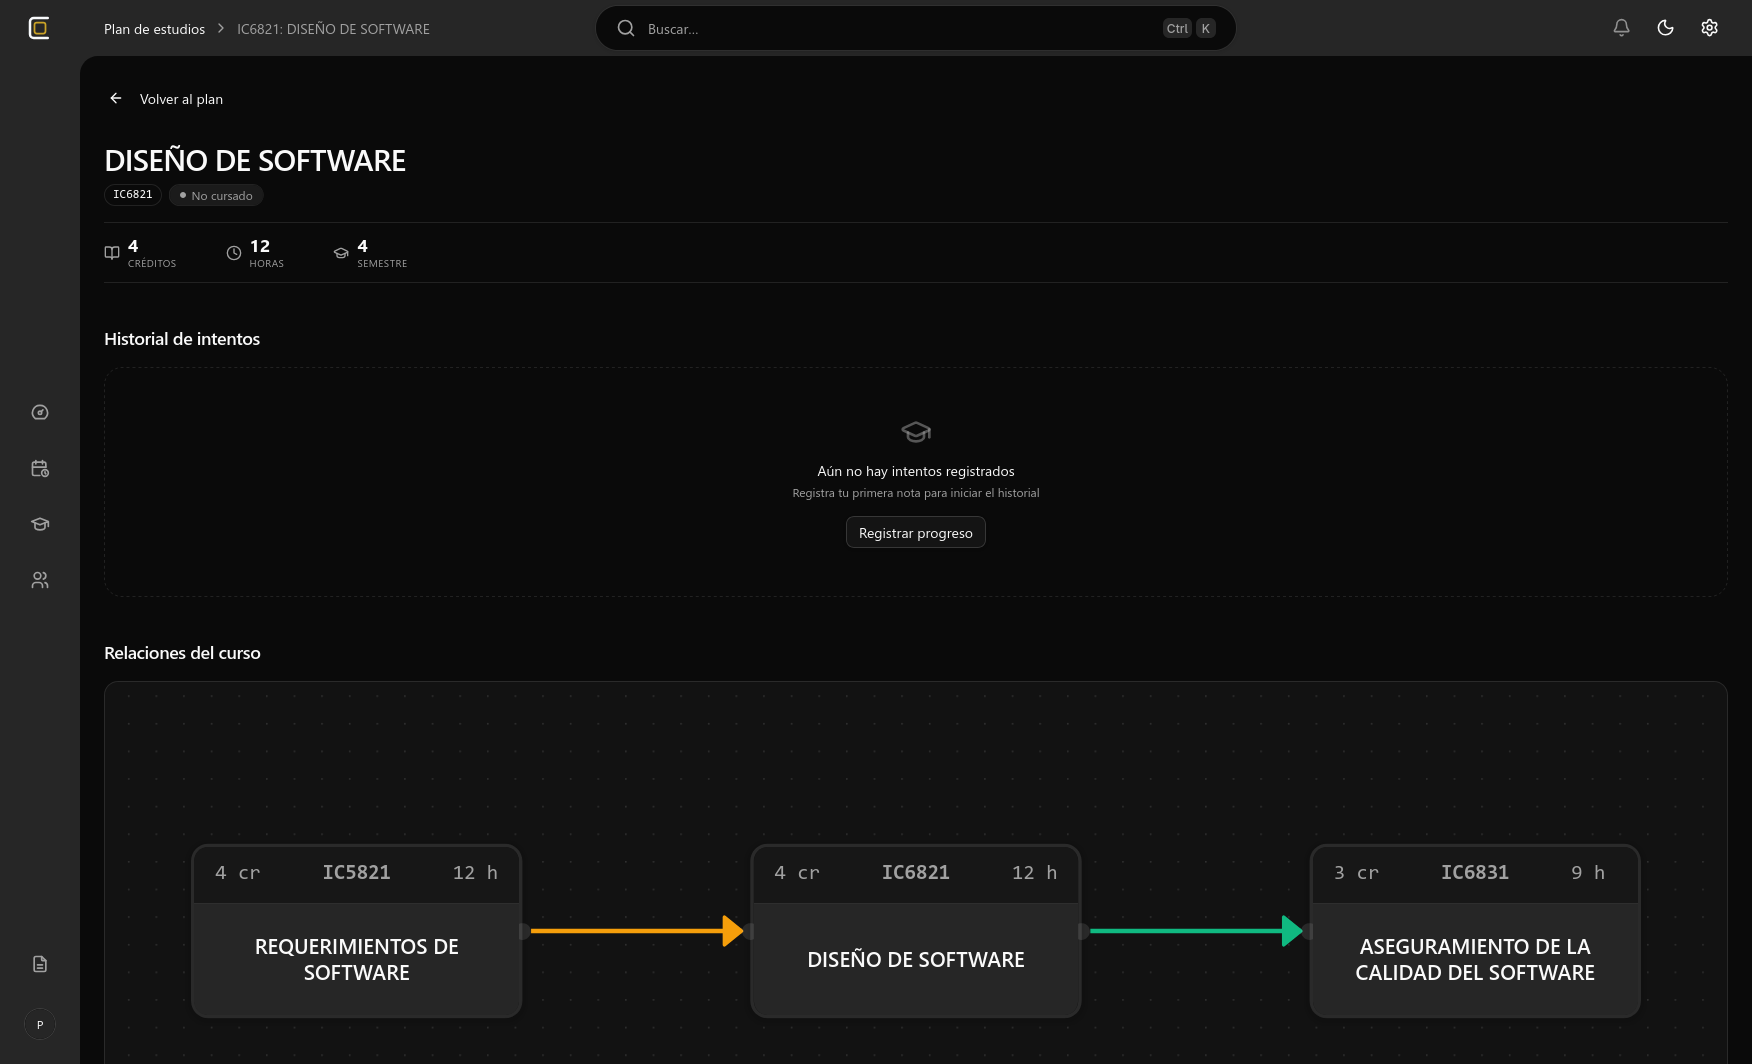
\includegraphics[width=0.92\textwidth]{images/caso-prueba-curriculum-detalle-curso.png}
\caption{Visualización de información de curso en la malla curricular}
\label{fig:curriculum-detalle}
\end{figure}

\subsubsection{CP-A-005 y CP-A-006: navegación y accesibilidad}

CP-A-005 verificó que las rutas principales se alcanzan en máximo 3 clics desde la aplicación autenticada, mientras que CP-A-006 complementó esta revisión mediante Lighthouse, con una puntuación de 94 en accesibilidad para la malla curricular. Adicionalmente, la evaluación de curriculum reportó 79 en rendimiento, 100 en buenas prácticas y 100 en SEO.

\begin{figure}[H]
\centering
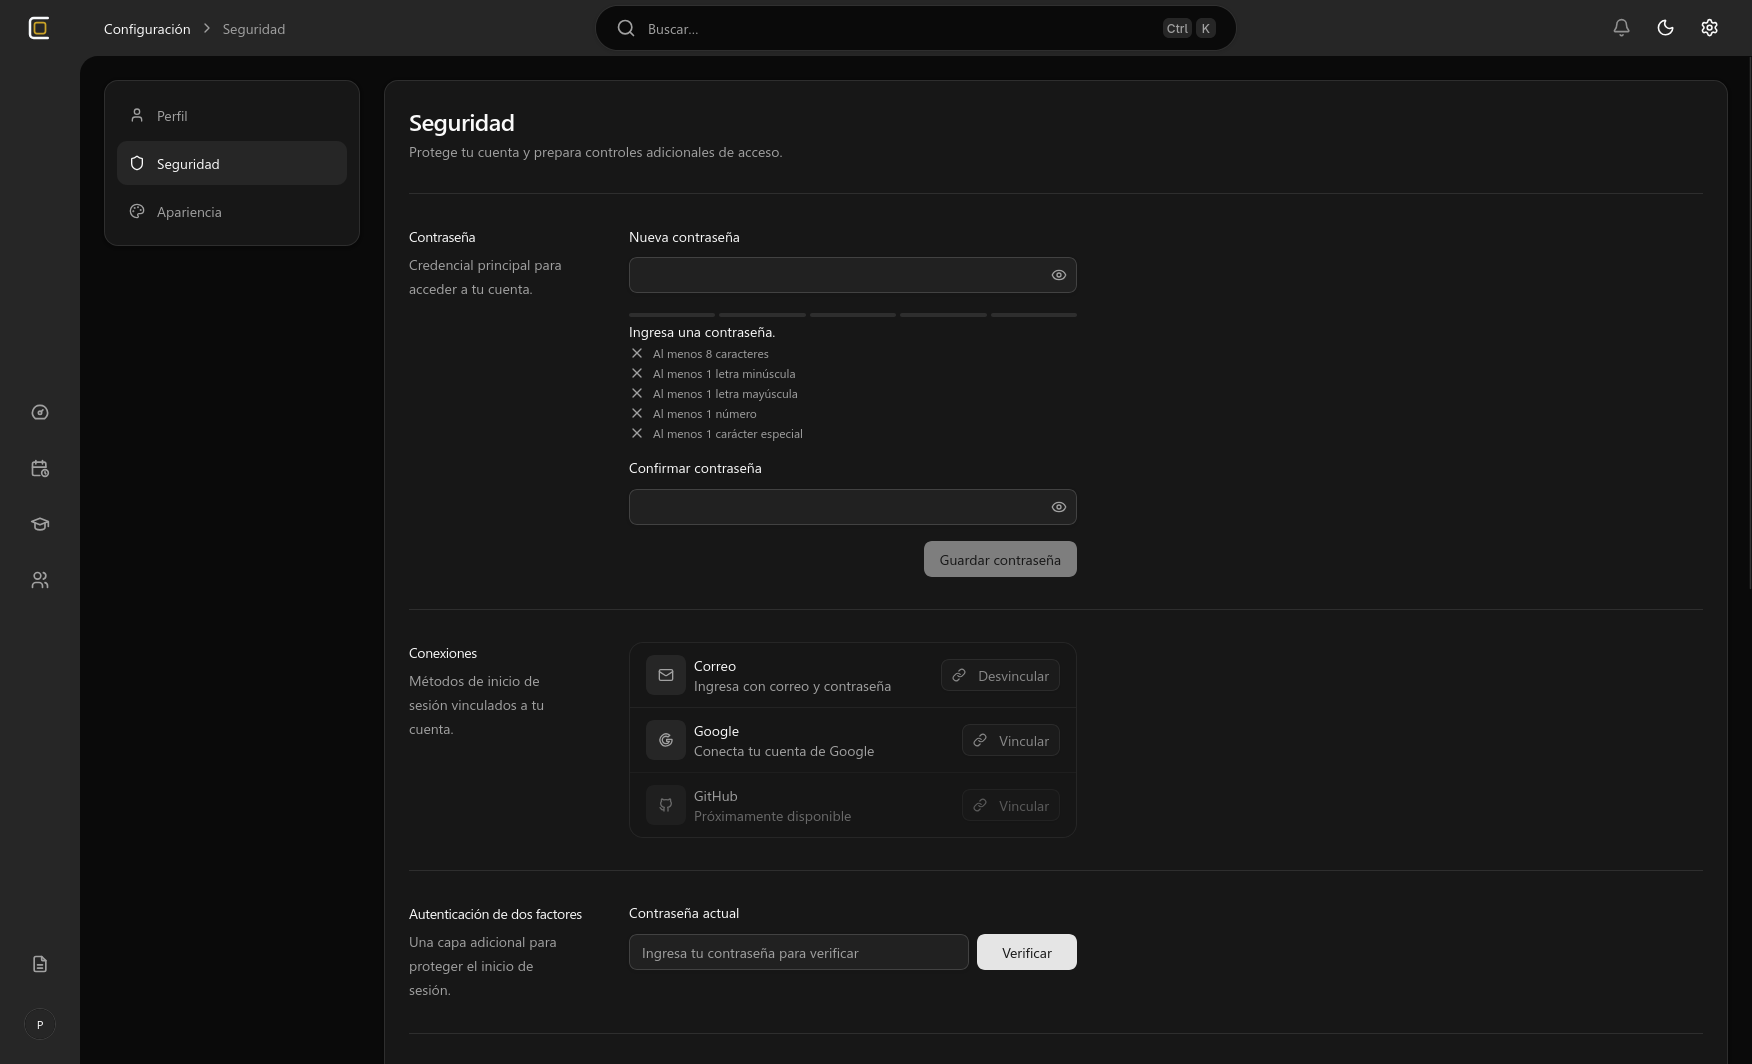
\includegraphics[width=0.92\textwidth]{images/caso-prueba-navegacion-tres-clics.png}
\caption{Validación de navegación hacia rutas principales en máximo 3 clics}
\label{fig:navegacion-tres-clics}
\end{figure}

\subsubsection{CP-A-007: aceptación de usuario de navegación autenticada}

CP-A-007 validó que un usuario autenticado puede orientarse entre las secciones principales sin confusión y dentro del límite de navegación definido, y la evidencia muestra el cierre del flujo de aceptación asociado a las rutas principales del sistema.

\begin{figure}[H]
\centering
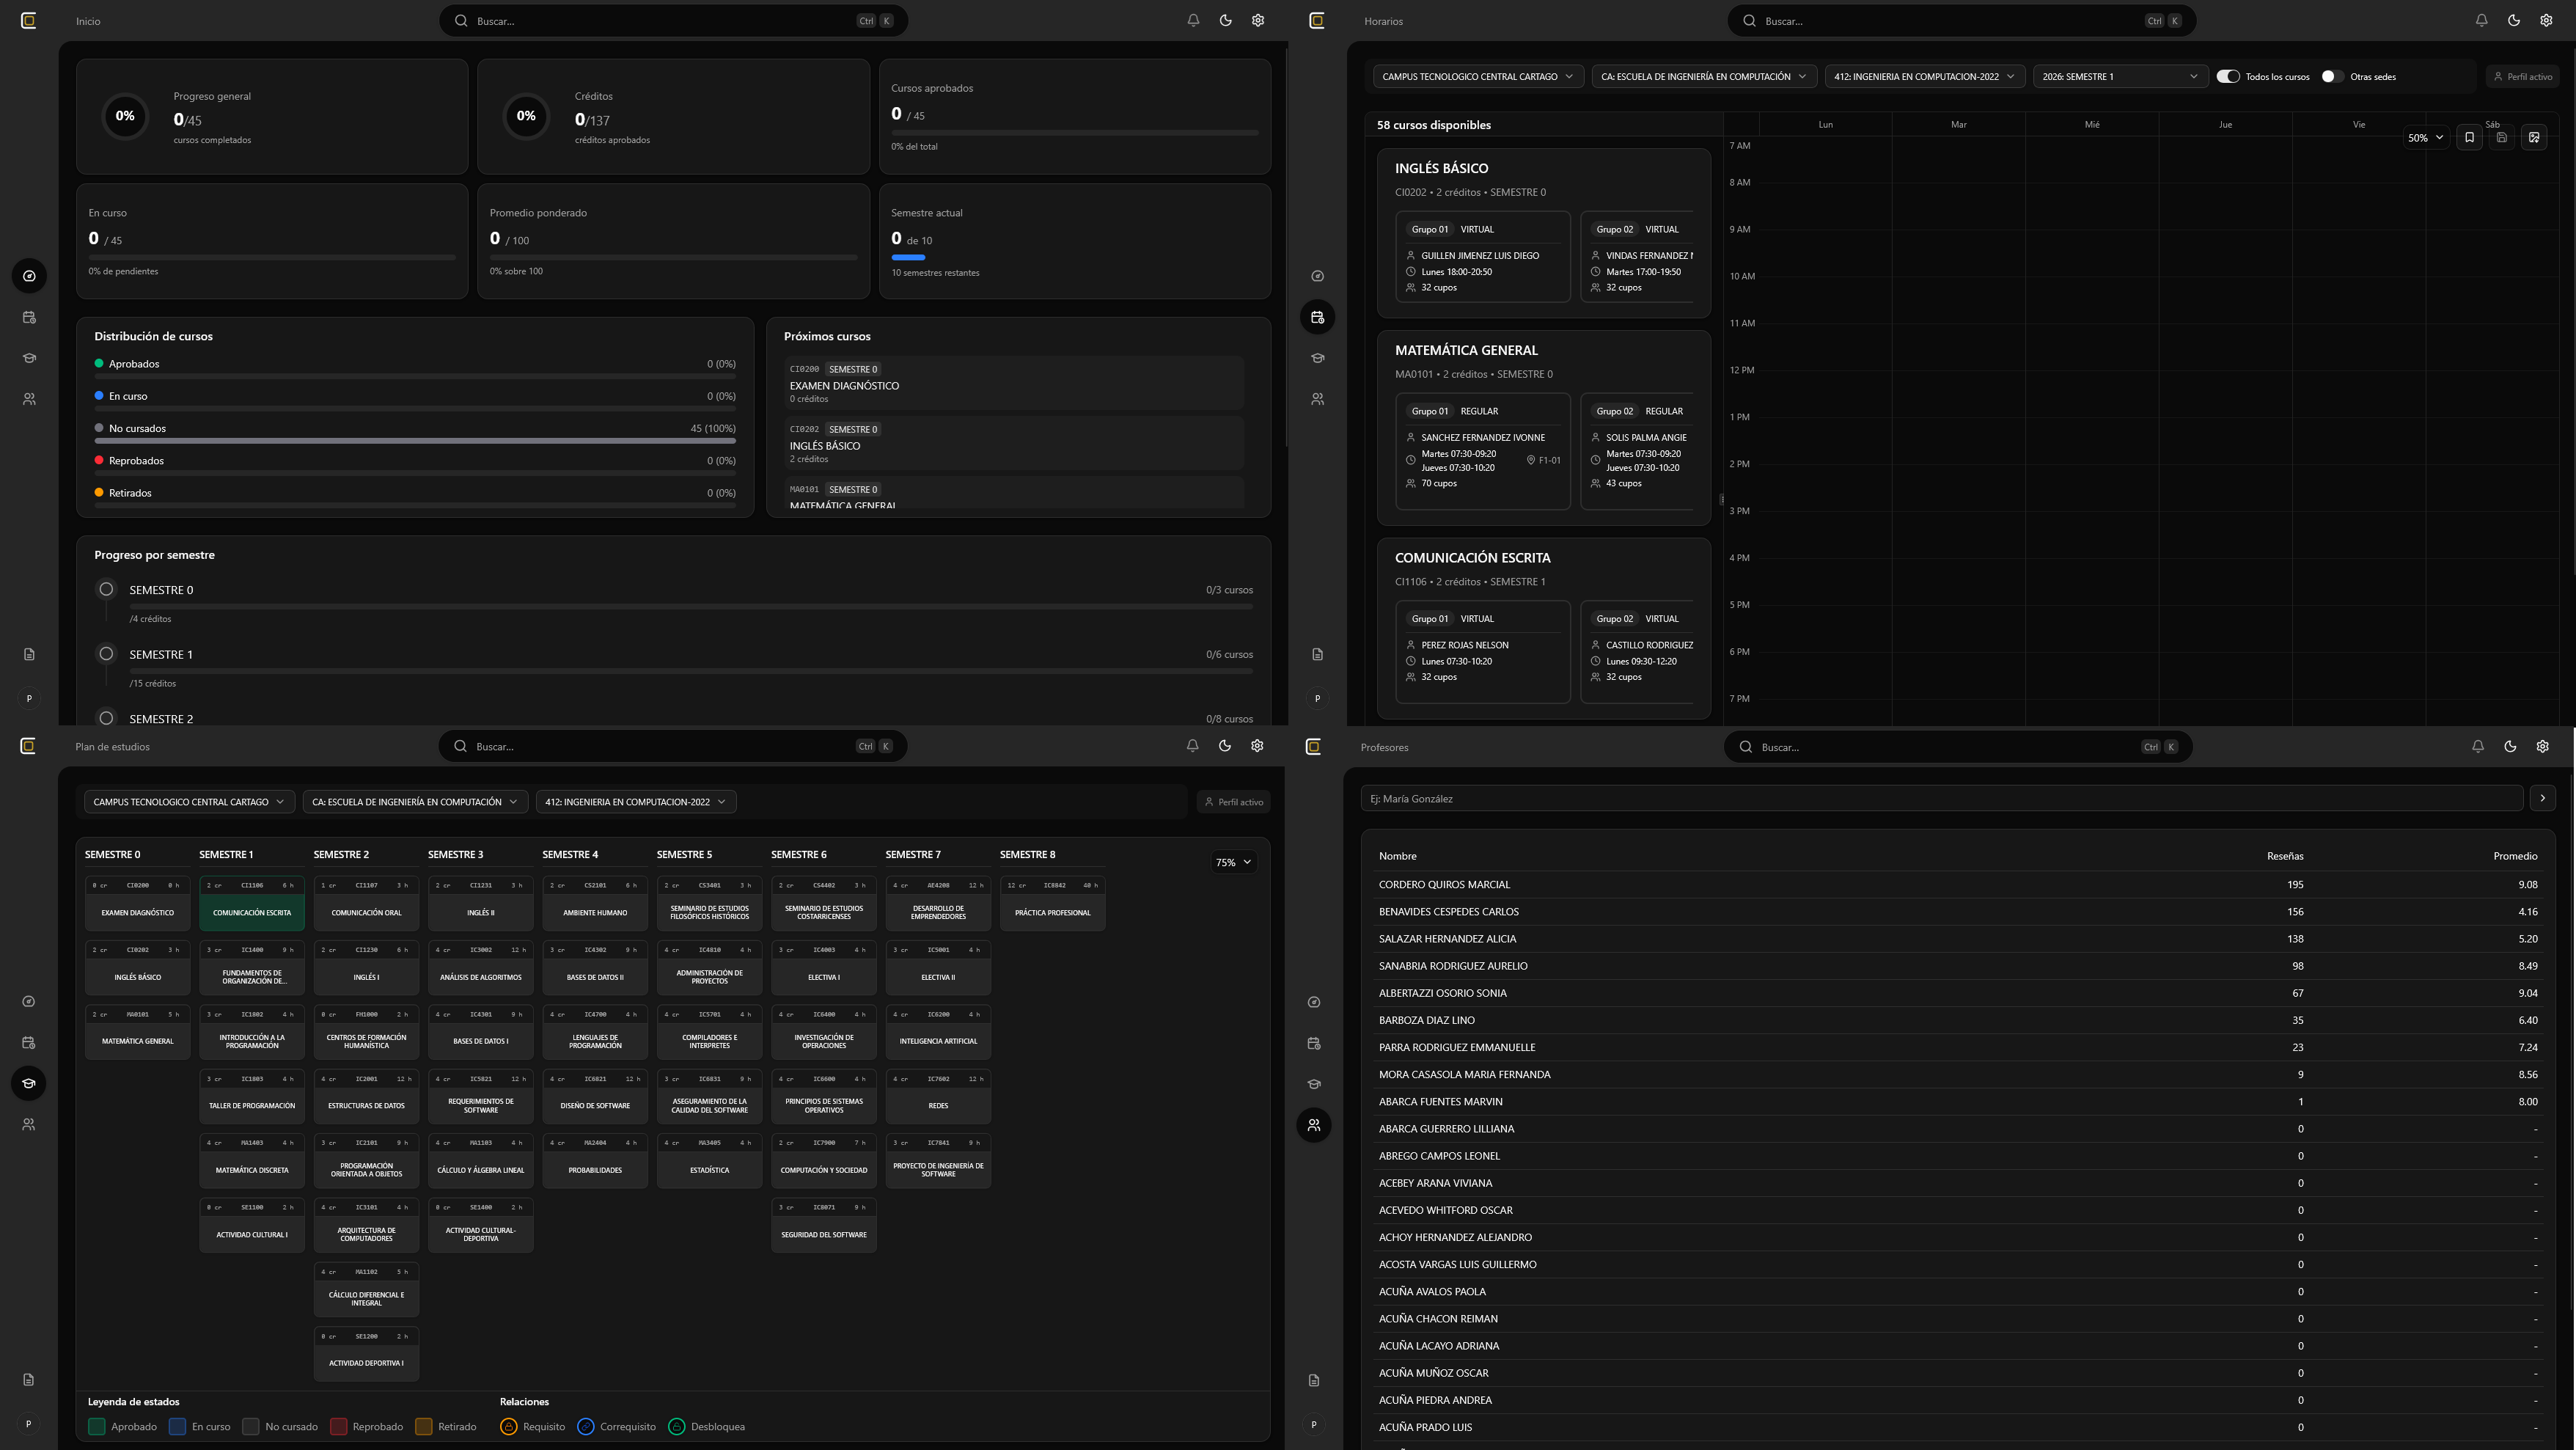
\includegraphics[width=0.92\textwidth]{images/aceptacion-usuario-navegacion-autenticada.png}
\caption{Aceptación de usuario sobre navegación autenticada entre secciones principales}
\label{fig:uat-navegacion}
\end{figure}

\subsection{Resumen consolidado de casos}

\begin{widepage}
\begin{longtable}{p{2.2cm} p{4.5cm} p{2.6cm} p{3.4cm} p{2.4cm} p{6.2cm}}
\caption{Resumen consolidado de casos de prueba ejecutados}\label{tab:casos-resumen}\\
\toprule
\textbf{ID} & \textbf{Nombre} & \textbf{Requisito} & \textbf{Tipo} & \textbf{Resultado} & \textbf{Resultado obtenido sintetizado} \\
\midrule
\endfirsthead
\toprule
\textbf{ID} & \textbf{Nombre} & \textbf{Requisito} & \textbf{Tipo} & \textbf{Resultado} & \textbf{Resultado obtenido sintetizado} \\
\midrule
\endhead
CP-M-001 & Acceso al creador de horarios & RF-M1 & Funcional & Aprobado & La ruta \texttt{schedule} cargó para el usuario demo y mostró cursos disponibles y calendario. \\
CP-M-002 & Agregar grupo al horario & RF-M1 & Funcional & Aprobado & El grupo \texttt{MA0101-01} apareció en el calendario semanal. \\
CP-M-003 & Guardar horario & RF-M1 & Integración & Aprobado & El diálogo permitió guardar el horario con el nombre definido. \\
CP-M-004 & Cargar horario guardado & RF-M1 & Sistema & Aprobado & El horario guardado apareció en la lista después de recargar. \\
CP-M-005 & Rendimiento del panel de resumen & RNF-M1 & Rendimiento & Aprobado & Se registró LCP de 1633 ms y CLS de 0.04 en \texttt{overview}. \\
CP-M-006 & Selección inválida o conflicto de horario & RF-M1 & Negativo & Aprobado & Los grupos con traslape se mostraron deshabilitados. \\
CP-M-007 & Carga ligera en ruta principal & RNF-M1 & Carga & Aprobado & Se completaron 30 solicitudes, sin fallos y con tiempo medio de 402.189 ms. \\
CP-M-008 & Prueba unitaria de lógica de horarios & RF-M1 & Unitario & Aprobado & Vitest ejecutó 4 pruebas unitarias y todas pasaron. \\
CP-M-009 & Aceptación de usuario del creador de horarios & RF-M1 & Aceptación & Aprobado & El flujo completo permitió entrar, agregar grupo, guardar y reutilizar horario. \\
CP-I-001 & Buscar profesor & RF-I1 & Funcional & Aprobado & Se abrió el detalle del profesor \texttt{CORDERO QUIROS MARCIAL}. \\
CP-I-002 & Consultar reseñas existentes & RF-I1 & Funcional & Aprobado & Se mostraron reseñas con datos y opciones de interacción. \\
CP-I-003 & Enviar reseña válida & RF-I1 & Funcional & Fallido & La aplicación rechazó una reseña válida con \texttt{Invalid review payload}. \\
CP-I-004 & Campos obligatorios vacíos & RF-I1 & Negativo & Aprobado & El formulario rechazó el envío y mostró mensaje de revisión de datos. \\
CP-I-005 & Intento de XSS & RNF-I1 & Seguridad & Aprobado & El payload XSS fue rechazado sin ejecución de script. \\
CP-I-006 & API de reseñas & RF-I1, RNF-I1 & API & Aprobado & Newman ejecutó 4 solicitudes y 14 aserciones sin fallos. \\
CP-I-007 & Aceptación de usuario del flujo de reseñas & RF-I1 & Aceptación & Fallido & La consulta funcionó, pero el envío de reseña válida no se completó. \\
CP-I-008 & Intento de SQL Injection & RNF-I1 & Seguridad & Aprobado & La entrada fue tratada como texto y no expuso errores ni datos no autorizados. \\
CP-A-001 & Login válido & RF-A1 & Funcional & Aprobado & La aplicación permitió acceder con credenciales válidas. \\
CP-A-002 & Login inválido & RF-A1 & Negativo & Fallido & El rechazo ocurrió con un mensaje incorrecto sobre formato de correo. \\
CP-A-003 & Onboarding académico & RF-A1 & Integración & Aprobado & El usuario demo ya tenía onboarding completado y redirigió correctamente. \\
CP-A-004 & Detalle de curso en la malla curricular & RNF-A1 & Funcional & Aprobado & Los cursos mostraron créditos, horas y semestre. \\
CP-A-005 & Navegación en máximo 3 clics & RNF-A1 & Usabilidad & Aprobado & Ninguna sección excedió los 3 clics. \\
CP-A-006 & Accesibilidad en la malla curricular & RNF-A1 & Accesibilidad & Aprobado & Lighthouse reportó 94 en accesibilidad. \\
CP-A-007 & Aceptación de usuario de navegación autenticada & RNF-A1 & Aceptación & Aprobado & Todas las rutas principales fueron accesibles para un usuario autenticado. \\
CP-A-008 & Control de acceso sin sesión & RF-A1 & Seguridad & Aprobado & Las rutas protegidas verificadas desplegaron bloqueos correctamente. \\
\bottomrule
\end{longtable}
\end{widepage}

\section{Defectos encontrados}

La gestión de defectos utilizó una escala de severidad y prioridad para distinguir problemas bloqueantes de problemas de experiencia o claridad, donde la severidad crítica se reservó para fallos que bloquean un flujo principal o exponen información sensible. La severidad alta se utilizó cuando una función importante se ve afectada y existe alternativa limitada, la severidad media correspondió a afectaciones parciales de experiencia o consistencia, y la severidad baja se aplicó a problemas visuales, texto, accesibilidad menor o mejoras.

\begin{widepage}
{\small
\setlength{\tabcolsep}{3pt}
\begin{longtable}{p{1.8cm} p{3.3cm} p{5.2cm} p{1.8cm} p{1.8cm} p{4.6cm} p{2cm} p{2cm}}
\caption{Registro formal de defectos}\label{tab:defectos}\\
\toprule
\textbf{ID} & \textbf{Título} & \textbf{Descripción} & \textbf{Sev.} & \textbf{Prior.} & \textbf{Resultado esperado} & \textbf{Estado} & \textbf{Resp.} \\
\midrule
\endfirsthead
\toprule
\textbf{ID} & \textbf{Título} & \textbf{Descripción} & \textbf{Sev.} & \textbf{Prior.} & \textbf{Resultado esperado} & \textbf{Estado} & \textbf{Resp.} \\
\midrule
\endhead
DEF-A-001 & Mensaje incorrecto en inicio de sesión & La prueba de login con credenciales inválidas retorna que el correo no tiene un formato válido, aunque el correo ingresado es correcto y el problema real corresponde a la contraseña o a credenciales inválidas. & Baja & Baja & El sistema debería indicar que la contraseña es incorrecta o que las credenciales son inválidas. & Abierto & Armando \\
DEF-I-001 & Envío de reseña válida rechazado & Al completar el formulario de reseña con datos aparentemente válidos, la aplicación rechaza el envío con el mensaje \texttt{Invalid review payload}, sin indicar qué campo específico causa el problema. & Alta & Alta & La reseña válida debería enviarse correctamente o quedar pendiente de aprobación con un mensaje claro. & Abierto & Isaac \\
\bottomrule
\end{longtable}
}
\end{widepage}

El defecto DEF-A-001 tiene bajo impacto operativo porque no permite acceso indebido y el control de autenticación continúa rechazando credenciales incorrectas, aunque deteriora la experiencia del usuario porque comunica una causa equivocada y puede inducir a modificar el correo en lugar de revisar la contraseña. Su corrección recomendada consiste en alinear la validación del mensaje con la causa real del rechazo o utilizar un mensaje genérico de credenciales inválidas.

El defecto DEF-I-001 tiene impacto alto porque afecta directamente un flujo funcional importante, dado que el módulo permite consultar profesores y abrir el formulario, pero el usuario no puede completar exitosamente el envío de una reseña válida. Además, el mensaje genérico dificulta identificar si el problema se encuentra en el curso, el periodo, el comentario, las calificaciones, la etiqueta o algún formato esperado por el backend, lo que incrementa el costo de diagnóstico y reduce la confianza en el flujo.

\section{Análisis de resultados}

Los resultados muestran un comportamiento sólido en el módulo de horarios, ya que la ruta \texttt{schedule} permitió ejecutar el flujo completo de creación, guardado y carga de horario, y además evitó conflictos al deshabilitar grupos con traslape. Esta combinación de funcionalidad positiva y prevención de errores respalda el cumplimiento de RF-M1, mientras que la presencia de pruebas unitarias sobre utilidades de calendario aumenta la confianza sobre la lógica de apoyo, aunque la cobertura reportada se limita al alcance de archivos probados y no debe interpretarse como cobertura global del sistema.

El rendimiento observado en \texttt{overview} también fue favorable dentro del umbral definido, dado que el LCP de 1633 ms cumple RNF-M1 y el CLS de 0.04 indica estabilidad visual aceptable en la medición realizada. Además, la carga ligera ejecutada con ApacheBench no produjo solicitudes fallidas, lo que sugiere respuesta estable bajo el escenario moderado aplicado, aunque el análisis debe interpretarse con prudencia porque se trató de una prueba acotada y no de una evaluación completa de capacidad o estrés.

En el módulo de profesores se observa una situación mixta porque la consulta de profesores, la visualización de reseñas, la apertura del formulario y las pruebas de seguridad tuvieron resultados favorables, mientras que las entradas XSS y SQL Injection no se ejecutaron ni expusieron errores técnicos, y Newman no registró fallos en las solicitudes evaluadas. Sin embargo, el rechazo de una reseña válida impide considerar aprobado el requisito funcional RF-I1, un resultado especialmente relevante porque afecta una acción central del módulo y no solo una validación periférica.

La autenticación y el onboarding cumplieron el flujo principal, ya que el usuario demo pudo iniciar sesión, la redirección de onboarding completado funcionó y las rutas protegidas verificadas no quedaron expuestas sin sesión válida. El defecto encontrado en login corresponde a calidad de mensaje y no a ruptura del control de acceso, por lo que RF-A1 se considera aprobado con defecto menor asociado. Asimismo, la malla curricular y la navegación autenticada cumplieron RNF-A1, ya que las rutas principales fueron accesibles en máximo 3 clics y la puntuación de accesibilidad de curriculum superó el umbral definido.

\section{Evaluación general de calidad}

\subsection{Cumplimiento funcional}

El cumplimiento funcional fue alto en horarios, autenticación, onboarding y navegación curricular, aunque el principal incumplimiento se concentró en el envío de reseñas, que impide completar el flujo funcional del módulo \texttt{professors}. Por esta razón, el sistema no puede considerarse completamente conforme dentro del alcance total, aunque sí presenta módulos específicos con cumplimiento satisfactorio.

\subsection{Calidad no funcional}

Los atributos no funcionales evaluados muestran resultados positivos dentro de los escenarios aplicados, ya que el panel de resumen cumplió el criterio de carga menor a 2 segundos, la accesibilidad de curriculum alcanzó 94 y la navegación entre secciones principales se mantuvo dentro del límite de 3 clics. En seguridad de entradas, las pruebas de XSS y SQL Injection no evidenciaron ejecución de código, exposición de errores SQL ni acceso indebido a datos.

\subsection{Deuda técnica y mantenibilidad}

La revisión estática con oxlint no reportó hallazgos bloqueantes en los componentes revisados de \texttt{schedule}, \texttt{calendar} ni en \texttt{calendar-utils.ts}, aunque como deuda técnica potencial se identifica la revisión de oportunidades de optimización de renderizado, ya que la traza de rendimiento atribuye una parte importante del LCP a demora de renderizado. También queda pendiente mejorar la validación y mensajería del formulario de reseñas, así como alinear la retroalimentación de login inválido con la causa real del rechazo.

Para el módulo \texttt{professors} no se contó con acceso directo a todo el código fuente de Claustrum, por lo que la revisión estática se limitó a los artefactos disponibles en el repositorio de QA, la colección Newman, los reportes generados y el comportamiento observable de la aplicación desplegada. Esta limitación impide confirmar internamente si el defecto DEF-I-001 proviene de transformación de datos en frontend, contrato de API, validación del backend o configuración de campos requeridos.

\subsection{Riesgos identificados}

El principal riesgo operativo de las pruebas automatizadas es la dependencia de datos externos o cambiantes, ya que si cambian cursos, profesores, grupos o disponibilidad académica, los flujos E2E pueden requerir ajustes en datos de prueba. También existe dependencia del usuario demo y de su estado, especialmente para horarios guardados y onboarding completado, mientras que en la API de reseñas un cambio en endpoints RPC de Supabase, parámetros o políticas de acceso podría invalidar la colección Newman y exigir mantenimiento.

Desde la perspectiva del producto, el mayor riesgo funcional está en el módulo de reseñas, debido a que si un estudiante puede consultar información pero no enviar una reseña válida, el módulo pierde una parte importante de su propósito colaborativo. Además, el mensaje \texttt{Invalid review payload} no orienta al usuario ni al equipo de soporte, por lo que podría aumentar reportes repetidos y dificultar el diagnóstico.

\section{Conclusiones}

El proceso de aseguramiento de calidad permitió verificar que Claustrum cumple de manera satisfactoria varios flujos críticos dentro del alcance evaluado, pues el creador de horarios funciona para el acceso autenticado, la selección de grupos, el guardado, la carga posterior y la prevención de conflictos. Además, el panel de resumen cumplió el umbral de rendimiento establecido, y la navegación autenticada hacia rutas principales se mantuvo dentro del límite de usabilidad definido.

La autenticación, el onboarding y el control de acceso presentaron resultados adecuados para los escenarios evaluados, ya que el defecto detectado en login no compromete el bloqueo de credenciales inválidas, aunque sí debe corregirse para mejorar claridad y consistencia de la experiencia. La malla curricular mostró información académica relevante y alcanzó una puntuación de accesibilidad aceptable, por lo que el requisito no funcional asociado se considera aprobado.

El módulo de profesores requiere atención prioritaria porque, aunque la consulta de profesores y reseñas funciona y las pruebas de seguridad no mostraron ejecución de payloads maliciosos, el envío de una reseña válida falla con un mensaje genérico. Este comportamiento afecta directamente el requisito RF-I1 y representa el defecto más significativo del proyecto, por lo que el sistema evaluado muestra calidad favorable en la mayoría de módulos, pero mantiene una brecha funcional importante en el flujo de reseñas.

\section{Recomendaciones}

Se recomienda corregir prioritariamente el defecto DEF-I-001, de modo que la aplicación acepte reseñas válidas o, si existe una regla adicional no visible para el usuario, la comunique mediante mensajes específicos por campo. También conviene revisar el contrato entre frontend y backend para confirmar nombres de campos, tipos de datos, formato de periodo, curso seleccionado, rangos de calificación, etiquetas y estado esperado de aprobación.

Para DEF-A-001 se recomienda reemplazar el mensaje incorrecto por una retroalimentación coherente con credenciales inválidas, preferiblemente mediante un mensaje genérico que no revele información sensible y que indique al usuario revisar correo y contraseña. Esta solución mantiene seguridad y mejora la experiencia sin requerir información detallada sobre cuál credencial falló.

Se recomienda mantener datos de prueba estables para la automatización E2E, especialmente en profesores, cursos y horarios, y también conviene ejecutar periódicamente Lighthouse y Performance sobre \texttt{overview} y \texttt{curriculum}, ya que los resultados actuales son favorables pero pueden variar con cambios de datos, componentes o carga de recursos. Finalmente, la colección Newman debe mantenerse alineada con los endpoints reales de Supabase RPC utilizados por la aplicación.

\section{Anexos}

Se presentan las evidencias visuales por módulo, los reportes técnicos considerados durante la evaluación y los criterios de clasificación utilizados para registrar la severidad y prioridad de los defectos encontrados.

\subsection{Anexo A: evidencias visuales por módulo}

\begin{longtable}{p{3cm} p{4.2cm} p{7cm}}
\caption{Evidencias visuales utilizadas en la evaluación}\label{tab:anexo-evidencias}\\
\toprule
\textbf{Módulo} & \textbf{Casos relacionados} & \textbf{Evidencia documentada} \\
\midrule
\endfirsthead
\toprule
\textbf{Módulo} & \textbf{Casos relacionados} & \textbf{Evidencia documentada} \\
\midrule
\endhead
Schedule & CP-M-001, CP-M-002, CP-M-003, CP-M-004, CP-M-006, CP-M-009 & Acceso al creador de horarios, selección de grupo, guardado, carga posterior, prevención de conflictos y aceptación del flujo completo. \\
Overview & CP-M-005 & Captura del panel de resumen utilizado como base para la evaluación de rendimiento. \\
Professors & CP-I-001, CP-I-002, CP-I-003, CP-I-004, CP-I-005, CP-I-007, CP-I-008 & Consulta de profesor, reseñas existentes, rechazo de reseña válida, validación de campos obligatorios, prueba XSS, aceptación de usuario y prueba SQL Injection. \\
Auth & CP-A-001, CP-A-002, CP-A-008 & Inicio de sesión válido, mensaje incorrecto ante credenciales inválidas y control de acceso sin sesión activa. \\
Onboarding & CP-A-003 & Redirección correcta de usuario con configuración académica completada. \\
Curriculum y navegación & CP-A-004, CP-A-005, CP-A-007 & Visualización de información de cursos, navegación en máximo 3 clics y aceptación de usuario sobre rutas principales. \\
\bottomrule
\end{longtable}

\subsection{Anexo B: reportes de herramientas}

\begin{table}[H]
\centering
\caption{Reportes técnicos considerados como respaldo de resultados}
\label{tab:anexo-reportes}
\begin{tabularx}{\textwidth}{p{3.8cm} p{4.2cm} Y}
\toprule
\textbf{Herramienta} & \textbf{Reporte o resultado} & \textbf{Uso dentro del análisis} \\
\midrule
Performance y Lighthouse & LCP de 1633 ms, CLS de 0.04, accesibilidad 100, buenas prácticas 100 y SEO 66 en \texttt{overview}. & Sustenta la aprobación de RNF-M1 y permite identificar que el rendimiento observado cumple el umbral definido para el panel de resumen. \\
ApacheBench & 30 solicitudes, concurrencia 3, cero solicitudes fallidas, 7.46 solicitudes por segundo y tiempo medio total de 402.189 ms. & Complementa la evaluación de \texttt{overview} con una carga ligera controlada. \\
Vitest & 4 pruebas unitarias aprobadas sobre utilidades de calendario. & Respalda la lógica auxiliar relacionada con horarios y contribuye a la evaluación de RF-M1. \\
Newman & 4 solicitudes, 14 aserciones y cero fallos contra endpoints de reseñas. & Sustenta los resultados de API y seguridad del módulo \texttt{professors}. \\
Lighthouse en curriculum & Rendimiento 79, accesibilidad 94, buenas prácticas 100 y SEO 100. & Respalda la evaluación de accesibilidad y calidad observable en la malla curricular. \\
Playwright & Flujos automatizados asociados a horarios, profesores y curriculum. & Aporta evidencia de ejecución de extremo a extremo en rutas autenticadas y formularios evaluados. \\
\bottomrule
\end{tabularx}
\end{table}

\subsection{Anexo C: criterios de clasificación de defectos}

\begin{table}[H]
\centering
\caption{Criterios de severidad aplicados a defectos}
\label{tab:anexo-severidad}
\begin{tabularx}{\textwidth}{p{3cm} Y}
\toprule
\textbf{Severidad} & \textbf{Criterio utilizado} \\
\midrule
Crítica & Bloquea un flujo principal completo o expone información sensible. \\
Alta & Afecta una función importante y ofrece una alternativa limitada o poco clara. \\
Media & Afecta experiencia, consistencia o resultados parciales sin bloquear completamente el uso. \\
Baja & Corresponde a un problema visual, textual, de accesibilidad menor o de mejora de comunicación. \\
\bottomrule
\end{tabularx}
\end{table}

\begin{table}[H]
\centering
\caption{Criterios de prioridad aplicados a defectos}
\label{tab:anexo-prioridad}
\begin{tabularx}{\textwidth}{p{3cm} Y}
\toprule
\textbf{Prioridad} & \textbf{Criterio utilizado} \\
\midrule
Alta & Debe atenderse antes de una entrega porque afecta fuertemente el resultado o impide validar un requisito relevante. \\
Media & Debe documentarse y corregirse cuando se planifique mantenimiento del módulo afectado. \\
Baja & Puede gestionarse como mejora futura si no compromete el flujo principal ni la seguridad. \\
\bottomrule
\end{tabularx}
\end{table}

\end{document}
